\documentclass[11pt]{article}
\usepackage[T1]{fontenc}
\usepackage[utf8]{inputenc}
\usepackage{lmodern}
\usepackage[margin=1in]{geometry}
\usepackage{amsmath,amssymb,amsthm,mathtools}
\usepackage{microtype,booktabs,array,longtable,enumitem}
\usepackage{graphicx}
\usepackage[hidelinks]{hyperref}
\usepackage{xurl}
\hypersetup{pdftitle={Polynomial Curvature and Weight Dependence in Optimal Cardinality Hierarchies},pdfauthor={Wenyu Huang},pdfsubject={Working paper on excess-risk hierarchy bounds},pdfkeywords={Bregman divergence, cardinality hierarchy, polynomial curvature, proper loss}}
\usepackage{fancyhdr}
\setlength{\headheight}{14pt}
\pagestyle{fancy}\fancyhf{}
\fancyhead[L]{\small Curvature and cardinality hierarchies}
\fancyhead[R]{\small Phase 8 v2}
\fancyfoot[C]{\thepage}
\setlength{\parskip}{0.25em}
\setlength{\emergencystretch}{2em}
\renewcommand{\arraystretch}{1.15}
\newtheorem{theorem}{Theorem}[section]
\newtheorem{lemma}[theorem]{Lemma}
\newtheorem{proposition}[theorem]{Proposition}
\newtheorem{corollary}[theorem]{Corollary}
\theoremstyle{definition}\newtheorem{definition}[theorem]{Definition}
\theoremstyle{remark}\newtheorem{remark}[theorem]{Remark}
\newcommand{\ph}{\varphi}
\newcommand{\B}{B_{\ph}}
\newcommand{\D}{D_{\ph}}
\newcommand{\OPT}{\operatorname{OPT}}
\newcommand{\E}{\mathbb E}
\newcommand{\Var}{\operatorname{Var}}
\newcommand{\R}{\mathbb R}
\newcommand{\rd}{\,\mathrm d}
\newcommand{\detp}{\mathrm{det}}
\newcommand{\stp}{\mathrm{stoch}}
\newcommand{\norm}[1]{\left\lVert #1\right\rVert}
\newcommand{\abs}[1]{\left\lvert #1\right\rvert}
\title{Polynomial Curvature and Weight Dependence in Optimal Cardinality Hierarchies}
\author{Wenyu Huang\\\small University of California San Diego}
\date{Phase 8 v2\\7 October 2026}
\begin{document}
\maketitle
\begin{center}\begin{minipage}{0.93\textwidth}\small
\textbf{Status.} Originality has not been established. The proofs have undergone internal independent review, which is not external peer review. Classical tools and prior project results are identified explicitly. This manuscript makes no publication-priority claim.
\end{minipage}\end{center}
\begin{abstract}
We study the excess Jensen risk caused by requiring finite representations at different output capacities to form a hierarchy. Three degree regimes emerge for nonnegative polynomial curvature of degree at most $r$. For four equal source masses, the optimal deterministic and stochastic two-/three-output worst-case prices have sharp order $\Theta(r/\log r)$, uniformly over posterior spacing; a fixed interior quartet gives the matching lower order. Allowing the four masses and posterior gaps to vary with degree produces prices $\Omega(r^2/(\log r)^2)$, whereas the general two-capacity upper bound remains $O(r^2)$. For arbitrary finite source counts and positive weights, we prove a simultaneous all-capacity upper bound $O(r^2\log(r+2))$, improving the earlier coarse $O(r^4)$ estimate. The proof compares each oriented Bregman divergence with squared distance in the classical curvature coordinate $h=\int\sqrt{\varphi''}$, using degree-uniform constants, and then applies an established hierarchy theorem. The weighted four-state witnesses also give an all-capacity lower bound. We retain fixed-generator sufficient conditions, including finite-order curvature zeros and analyticity across the closed interval, and give reproducible numerical diagnostics with explicit small-denominator and stochastic-certification limits. The localization, Markov, curvature-coordinate, and hierarchy-transfer tools are classical; no priority claim, optimal unrestricted-weight order, nonvanishing absolute excess loss, or neural-training guarantee is asserted.
\end{abstract}

\section{The question and the boundaries of the results}
A flat representation with output capacity $k$ partitions a finite source into at most $k$ cells. Under a strictly proper binary loss, its excess Bayes risk is a scalar Jensen distortion. Separately optimal representations can be incompatible: a three-cell optimum need not refine a two-cell optimum. The hierarchy price asks how much multiplicative excess distortion is necessary when the smaller representation must be obtained by coarsening the larger one.

We distinguish a \emph{fixed} generator from a degree-indexed \emph{class} of generators, and fixed positive weights from weights allowed to degenerate with degree. For four equal masses, both deterministic and stochastic degree envelopes have sharp order $\Theta(r/\log r)$. The upper bound permits arbitrary posterior spacing, while a fixed equally spaced interior quartet supplies the lower order. Every fixed positive four-state weight vector has the same order, with constants depending on its weight ratio, by a routine comparison of nonnegative weighted Bregman sums.

The weight-uniform problem is different. Section~\ref{sec:ext-weights} constructs four-state instances of curvature degree $r=2n$ with inner masses $d_n^2$, where $d_n=(4\log n/n)^2$, whose deterministic and stochastic prices are $\Omega(r^2/(\log r)^2)$. Their posterior gaps vary as well, so this construction does not isolate the effect of masses alone. It rules out an absolute-constant extension of the equal-mass $O(r/\log r)$ theorem to arbitrary positive weights. The remaining two-capacity upper bound is $O(r^2)$.

For one hierarchy covering \emph{all} capacities, arbitrary positive weights, and arbitrary finite source counts, Section~\ref{sec:poly-allcap-new} proves the uniform bound
\[
256r^2K_r,\qquad K_r=2\log(64r^2)+\tfrac14.
\]
It improves the earlier $O(r^4)$ estimate by comparing each oriented divergence with squared distance in the classical curvature coordinate. The four-state weighted lower bound embeds in the all-capacity problem, but leaves its optimal degree order open.

\begin{table}[ht]
\centering\small
\begin{tabular}{@{}>{\raggedright\arraybackslash}p{0.27\textwidth}>{\raggedright\arraybackslash}p{0.38\textwidth}>{\raggedright\arraybackslash}p{0.28\textwidth}@{}}
\toprule
Curvature and weight regime & Source and hierarchy scope & Proved consequence \\
\midrule
Degree at most $r$; equal masses & Four states; arbitrary posterior spacing; capacities two and three & Both prices have envelope $\Theta(r/\log r)$ \\
Degree $r=4n$; equal masses & One fixed interior quartet; varying generators & Sequence prices $\sim r/(128\log r)$ and $\sim r/(256\log r)$ \\
Degree at most $r$; fixed positive weights & Four states; capacities two and three & $\Theta_p(r/\log r)$ by weight comparison \\
Degree at most $r$; arbitrary positive weights & Four states; capacities two and three & Lower $\Omega(r^2/(\log r)^2)$; upper $1+128r^2$ \\
Degree at most $r$; arbitrary positive weights & Arbitrary finite source; all capacities & Upper $256r^2K_r$; lower $\Omega(r^2/(\log r)^2)$ \\
Finitely many finite-order curvature zeros & One fixed generator; arbitrary positive weights and finite source; all capacities & At most $32C_\varphi/c_\varphi$ \\
Adjacent-interval mass comparison & Fixed constant $A$; arbitrary finite positive weights; all capacities & At most $4Q(1+Q)$, $Q=4(A+1)^2$ \\
Monotone curvature & Every source mass at least $\alpha$; all capacities & At most $32/\alpha$ \\
Positive interior curvature; eventual endpoint monotonicity & Fixed $C^2$ generator; four equal masses; capacities two and three & Finite supremum over posterior locations \\
\bottomrule
\end{tabular}
\caption{Claim domains. Prices refer to excess distortion. Ratio statements use positive flat denominators; all-capacity upper bounds also handle zero optima through cost inequalities. Deterministic upper bounds also bound stochastic price. $r$ always denotes curvature degree.}
\label{tab:scope}
\end{table}

The earlier Phase 7 working paper \cite[Section 4]{huang7} constructs one smooth generator with positive interior curvature, bounded curvature, and finite endpoint slopes whose four-equal-mass price diverges along a sequence of posterior configurations. It places successively weaker curvature gadgets at scales accumulating at the endpoints. That fixed smooth obstruction is prior project work. Sections~\ref{sec:finiteorder}--\ref{sec:endpoints} give sufficient conditions that preclude it and necessary endpoint conditions for it; these do not form a complete classification.

The proofs combine established hierarchy transfer with scalar curvature estimates. The coordinate $h$, Markov's inequality, Chebyshev growth and needles, outer Fej\'er--Riesz factorization, and random-table revelation have classical or prior-project antecedents. The quantitative comparisons and hierarchy consequences are proved here with their exact domains; Section~\ref{sec:provenance} records attribution and access limits. The numerical section checks finite examples and reports absolute denominator scales. It does not replace any proof or certify a global stochastic optimum by numerical search.

\section{Distortion and hierarchy definitions}
\label{sec:definitions}
Let $X$ take values in $\{1,\ldots,N\}$ with $p_i>0$ and $\sum_i p_i=1$. Let $x_i\in[0,1]$ be scalar posteriors, interpreted as $\mathbb P(Y=1\mid X=i)$ when a binary target is supplied. Unless stated otherwise, $\ph:[0,1]\to\R$ is continuously differentiable and strictly convex. For curvature statements it is $C^2$, and $g=\ph''\ge0$.

Define the oriented Bregman divergence
\begin{equation}
\B(x,y)=\ph(x)-\ph(y)-\ph'(y)(x-y).
\label{eq:bregman}
\end{equation}
For a partition $P$, put
\begin{equation}
\D(P)=\sum_i p_i\ph(x_i)-\sum_{C\in P}p_C\ph(m_C),\qquad
p_C=\sum_{i\in C}p_i,\quad m_C=\frac{\sum_{i\in C}p_ix_i}{p_C}.
\label{eq:distortion}
\end{equation}
For a single cell, $\D(C)$ means its contribution to this sum, with the original, unnormalized source weights. The flat optimum $\OPT_k$ is the minimum of $\D(P)$ over partitions with at most $k$ cells. Refinement never increases distortion. Exact cell counts can be supplied by splitting cells when $k\le N$.

A deterministic hierarchy $H=(H_k)_{k=1}^N$ has $H_{k+1}$ refining $H_k$ and $|H_k|\le k$. Its price is the smallest $c$ satisfying $\D(H_k)\le c\OPT_k$ at every capacity. This cost-inequality definition also handles zero optima. When ratios are used, only capacities with $\OPT_k>0$ are included, with the additional requirement of zero hierarchical cost at a zero optimum. A two-level hierarchy with capacities $k<\ell$ is defined in the same way using just those levels. For four source states with positive weights, write
\begin{equation}
\rho_{\ph,\detp}=\min_{H_3\succeq H_2}\max\left\{
\frac{\D(H_2)}{\OPT_2},\frac{\D(H_3)}{\OPT_3}\right\},
\label{eq:detprice}
\end{equation}
where $H_3\succeq H_2$ denotes refinement, and both denominators are positive.

For a channel $X\to Z$, define
\begin{equation}
\D(Z)=\E\ph(x_X)-\E\ph\bigl(\E[x_X\mid Z]\bigr).
\label{eq:channel}
\end{equation}
A stochastic two-level hierarchy is a degradation chain $X\to Z_\ell\to Z_k$ with the indicated output budgets. Its price $\rho_{\ph,\stp}$ is the infimum of the corresponding maximum ratio. No public randomization variable is supplied to the predictor. In the binary interpretation, one can append $Y-X$ to the chain. A stochastic all-capacity hierarchy is a chain $X\to Z_N\to Z_{N-1}\to\cdots\to Z_1$ with $|Z_k|\le k$ and the same cost-inequality convention at zero optima. Every deterministic hierarchy is admissible in the corresponding stochastic model.

\begin{lemma}[Integral and centroid identities]
\label{lem:identities}
For $u<v$,
\begin{align}
\B(v,u)&=\int_u^v(v-t)g(t)\rd t,&
\B(u,v)&=\int_u^v(t-u)g(t)\rd t,\label{eq:integrals}\\
S_\ph(u,v)&:=\B(u,v)+\B(v,u)=(v-u)\int_u^v g(t)\rd t.\label{eq:symmetric}
\end{align}
For every cell $C$ and center $q\in[0,1]$,
\begin{equation}
\sum_{i\in C}p_i\B(x_i,q)=\D(C)+p_C\B(m_C,q).
\label{eq:centroid}
\end{equation}
In particular, the ordinary weighted arithmetic mean $m_C$ minimizes the left side.
\end{lemma}
\begin{proof}
Integrating $\ph''$ twice gives \eqref{eq:integrals}, and addition gives \eqref{eq:symmetric}. Expanding \eqref{eq:bregman}, subtracting the expression centered at $m_C$, and using $\sum_{i\in C}p_i(x_i-m_C)=0$ gives \eqref{eq:centroid}. Strict convexity makes its final term nonnegative, with equality precisely when $q=m_C$.
\end{proof}

\begin{lemma}[Stochastic flat optima]
\label{lem:flat}
For every output budget $k$, the infimum of \eqref{eq:channel} over all channels with at most $k$ outputs equals $\OPT_k$.
\end{lemma}
\begin{proof}
Any stochastic encoder can be generated by a random function table $U$, independent of $X$: for each possible input draw its output according to that row of the channel, and reveal only the output corresponding to the realized input. Conditional on $U$, the encoder is deterministic with at most $k$ outputs. Conditional Jensen gives
\[
\E\ph(\E[x_X\mid Z])\le \E\ph(\E[x_X\mid Z,U]),
\]
so $\D(Z)\ge\E_U\D(Z\mid U)\ge\OPT_k$. Conversely, a deterministic flat minimizer is a channel. Thus randomization does not change the flat denominators used throughout this paper.
\end{proof}

The Bregman centroid interpretation is classical \cite{banerjee}. Proper-loss interpretations are also classical \cite{gneiting,reid}. Positive rescaling of $\ph$ scales all distortions and leaves every price unchanged; adding an affine function leaves every distortion unchanged.

\begin{theorem}[Polynomial degree regimes]
\label{thm:main}
Let the nonnegative nonzero polynomial curvature have degree at most $r$.
\begin{enumerate}[label=(\roman*),leftmargin=*]
\item For four equal masses, the deterministic and stochastic two-/three-output worst-case prices are $\Theta(r/\log r)$ as $r\to\infty$, uniformly over posterior locations.
\item For four arbitrary positive masses, there are absolute constants $c>0$ and $r_0$ such that their envelopes satisfy
\[
c\frac{r^2}{(\log r)^2}\le\widehat C_r^{\stp}
\le\widehat C_r^{\detp}\le1+128r^2\qquad(r\ge r_0).
\]
\item For arbitrary finite source counts and positive weights, a single deterministic hierarchy has factor at most $256r^2K_r$ at every capacity, where $K_r=2\log(64r^2)+1/4$ for $r\ge1$. The same upper bound holds stochastically. The worst-case all-capacity prices in both models are at least $cr^2/(\log r)^2$ for large $r$. Constant curvature admits factor $32$.
\end{enumerate}
All degree envelopes allow the generator to vary. In (ii) and the all-capacity lower bound, weights and posterior gaps may also vary. No sharp order is asserted for these broader regimes.
\end{theorem}
\begin{proof}
Part (i) combines Theorems~\ref{thm:logupper} and \ref{thm:lower}.
Part (ii) combines Theorems~\ref{thm:polyupper} and \ref{thm:ext-weightdegenerate}.
Theorem~\ref{thm:poly-allcap-new} proves the upper bound in (iii), and Corollary~\ref{cor:ext-allcap} embeds the four-state witnesses at all capacities.
\end{proof}

\section{Transferring flat approximations to a hierarchy}
\label{sec:transfer}
We use the following established augmentation principle. It is the framework of Lin, Nagarajan, Rajaraman, and Williamson \cite{lin}, checked through the primary restatement in Gro\ss wendt \cite[Theorem 2.11, p.~29]{grosswendt}; the original Lin full text was not accessible for this review. Its parameter names vary between sources; here they are fixed by the displayed inequality.

\begin{theorem}[Classical augmentation principle]
\label{thm:augmentation}
Suppose a refinement-monotone clustering cost has the following property: for each partition $P$ and each smaller desired capacity $k$, a coarsening $P'$ with at most $k$ cells satisfies
\begin{equation}
D(P')\le\gamma D(P)+\delta\OPT_k,\qquad \gamma,\delta\ge1.
\label{eq:augment}
\end{equation}
Then there exists a hierarchy at all capacities with approximation factor at most $4\gamma\delta$.
\end{theorem}
This theorem is invoked as a published ingredient, not proved or claimed as a new result here. Hierarchical location and clustering approximations have an extensive prior literature, including Plaxton \cite{plaxton} and Arutyunova and R\"oglin \cite{arutyunova}. The factor-$32$ squared-Euclidean application is recorded in \cite[Lemma 2.13, pp.~30--31; Theorem 1.2, p.~32]{grosswendt}. We give the short positive-real-weight extension needed below.

\begin{lemma}[Weighted Hilbert-space transfer]
\label{lem:hilbert}
For any finite collection of points in a real Hilbert space, with arbitrary positive weights, an all-capacity squared-distance hierarchy exists with factor at most $32$.
\end{lemma}
\begin{proof}
Let $M$ be one cell of a fine partition, with total weight $W$ and centroid $m$. Let $c_1,\ldots,c_k$ be target centers, and assign each point $x_i$ to a closest center $c_{a(i)}$. The elementary inequality $\|u+v\|^2\le2\|u\|^2+2\|v\|^2$ gives
\begin{align*}
W\min_j\|m-c_j\|^2
&\le\sum_{i\in M}p_i\|m-c_{a(i)}\|^2\\
&\le 2\sum_{i\in M}p_i\|m-x_i\|^2
 +2\sum_{i\in M}p_i\|x_i-c_{a(i)}\|^2.
\end{align*}
Writing $V(M)=\sum_{i\in M}p_i\|x_i-m\|^2$, the squared-distance centroid identity yields
\[
\min_j\sum_{i\in M}p_i\|x_i-c_j\|^2
\le3V(M)+2\sum_{i\in M}p_i\|x_i-c_{a(i)}\|^2.
\]
Assign each fine cell to its minimizing target center and merge all cells assigned to the same center. Optimizing the centroid of each merged cell only decreases cost. Summing and weakening $3V(M)$ to $4V(M)$ proves \eqref{eq:augment} with $(\gamma,\delta)=(4,2)$ when the target partition is flat optimal. Theorem~\ref{thm:augmentation} gives $32$. Every calculation occurs in the finite-dimensional affine span of the input points, so the same proof applies in a Hilbert space. No rationality or replication assumption on the weights is used.
\end{proof}

A second transfer exploits the Bregman centroid identity directly.
\begin{proposition}[An oriented three-point sufficient condition]
\label{prop:qt}
Suppose that, for some $Q\ge1$ and every $x,u,v\in[0,1]$,
\begin{equation}
\B(u,v)\le Q\{\B(x,u)+\B(x,v)\}.
\label{eq:qt}
\end{equation}
Then all capacities admit a deterministic hierarchy of factor at most $4Q(1+Q)$. For any two capacities $k<\ell$, a hierarchy exists with price at most $1+2Q$, for arbitrary finite positive source weights. These are also stochastic upper bounds.
\end{proposition}
\begin{proof}
Let $P$ be the fine partition and $O$ a target partition with at most $k$ cells and centroids $q_1,\ldots,q_k$. For each fine cell $C$, choose a target centroid minimizing $\B(m_C,q_j)$. Let $q(i)$ be the centroid assigned to input $i$ by $O$. Then
\begin{align*}
p_C\min_j\B(m_C,q_j)
&\le\sum_{i\in C}p_i\B(m_C,q(i))\\
&\le Q\sum_{i\in C}p_i\{\B(x_i,m_C)+\B(x_i,q(i))\}.
\end{align*}
Merge fine cells assigned to the same target centroid. By \eqref{eq:centroid}, evaluating at that target centroid and then optimizing the merged centroid gives
\begin{equation}
\D(P')\le(1+Q)\D(P)+Q\D(O).
\label{eq:nesting}
\end{equation}
Theorem~\ref{thm:augmentation} gives the all-capacity bound. For two capacities, choose $P$ flat optimal at $\ell$ and $O$ flat optimal at $k$. Since $\OPT_\ell\le\OPT_k$, the coarse ratio is at most $1+2Q$, and the fine ratio is one. Deterministic hierarchies are stochastic admissible, and Lemma~\ref{lem:flat} identifies their flat denominators.
\end{proof}

\section{Finite-order curvature zeros and analytic generators}
\label{sec:finiteorder}
A positive lower bound on $g$ immediately compares $\B$ with squared Euclidean distance in the original posterior coordinate. The next result permits curvature to vanish at finitely many points. The relevant coordinate is instead the integral of the square root of curvature.

\begin{theorem}[Finite-order curvature comparison]
\label{thm:finiteorder}
Assume $g\ge0$ is continuous on $[0,1]$, is positive except at finitely many points $z$, and at each zero satisfies
\begin{equation}
c_z|t-z|^{m_z}\le g(t)\le C_z|t-z|^{m_z}
\label{eq:finiteorder}
\end{equation}
on a sufficiently small available one-sided or two-sided neighborhood, where $0<c_z\le C_z<\infty$ and $m_z\ge0$. Put
\[
h(x)=\int_0^x\sqrt{g(t)}\rd t.
\]
There are constants $0<c_\ph\le C_\ph<\infty$, depending on this fixed generator, such that
\begin{equation}
c_\ph|h(x)-h(y)|^2\le\B(x,y)\le C_\ph|h(x)-h(y)|^2
\label{eq:hcompare}
\end{equation}
for every $x,y\in[0,1]$. Every finite source with arbitrary positive weights admits an all-capacity deterministic hierarchy of factor at most $32C_\ph/c_\ph$. The same bound holds for stochastic price.
\end{theorem}
\begin{proof}
The map $h$ is continuous and strictly increasing. Away from the diagonal $x=y$, the numerator and denominator of $\B(x,y)/|h(x)-h(y)|^2$ are continuous and positive. Their ratio is therefore bounded above and away from zero on compact subsets avoiding the diagonal. Near a point where $g>0$, its uniform continuity and \eqref{eq:integrals} imply that this ratio tends to $1/2$ as both arguments approach that point.

It remains to control both orientations near a zero $z$. Suppose $x<y$ and their interval is contained in the neighborhood in \eqref{eq:finiteorder}. Set $L=y-x$ and $a=(z-x)/L$. The substitution $t=x+Ls$ shows that the model for $\B(y,x)/|h(y)-h(x)|^2$ is
\begin{equation}
R_m(a)=\frac{\int_0^1(1-s)|s-a|^m\rd s}
{\left(\int_0^1|s-a|^{m/2}\rd s\right)^2}.
\label{eq:modelratio}
\end{equation}
The actual ratio $\B(y,x)/|h(y)-h(x)|^2$ lies between $(c_z/C_z)R_{m_z}(a)$ and $(C_z/c_z)R_{m_z}(a)$. For $\B(x,y)$ replace $1-s$ by $s$. Each model ratio is continuous and strictly positive for every finite real $a$. Dividing its numerator and denominator by $|a|^m$ shows that it tends to $1/2$ as $a\to\pm\infty$. It consequently has a positive infimum and a finite supremum over all $a\in\R$. A finite cover of the diagonal by the positive-curvature and zero neighborhoods, combined with the off-diagonal compactness argument, proves \eqref{eq:hcompare}.

For a cell $C$, minimize \eqref{eq:hcompare} after summing with weights $p_i$. Since $h([0,1])$ is an interval containing all transformed data, its weighted arithmetic mean belongs to that interval. Hence
\[
\min_q\sum_{i\in C}p_i|h(x_i)-h(q)|^2
=\sum_{i\in C}p_i|h(x_i)-\overline h_C|^2,
\quad
\overline h_C=\frac{\sum_{i\in C}p_ih(x_i)}{p_C}.
\]
The centroid identity then gives $c_\ph V_h(P)\le\D(P)\le C_\ph V_h(P)$ for every partition. Notice that this argument minimizes over the center before comparing; it does not assert $h(m_C)=\overline h_C$. Apply Lemma~\ref{lem:hilbert} to the transformed points and compare the flat minima. This gives the claimed hierarchy factor.
\end{proof}

\begin{corollary}[Analyticity on a neighborhood of the closed interval]
\label{cor:analytic}
If $\ph$ is strictly convex on $[0,1]$ and real analytic on an open neighborhood of $[0,1]$, the conclusion of Theorem~\ref{thm:finiteorder} holds.
\end{corollary}
\begin{proof}
The analytic function $g=\ph''$ is nonnegative on $[0,1]$ and not identically zero. Its zeros in this compact interval are finite; otherwise an accumulation point in the analytic neighborhood would force it to vanish identically. The first nonzero Taylor coefficient at each zero supplies the two-sided bounds \eqref{eq:finiteorder} on the available neighborhood. Interior orders are even; an endpoint order need not be even when only the interval side is considered.
\end{proof}

For example, $\ph(x)=(x-1/2)^4$ has an interior curvature zero and still satisfies the theorem. The corollary is a \emph{fixed-generator} statement. It gives neither a uniform constant over analytic generators nor a conclusion from analyticity only on $(0,1)$.

The Hessian-root coordinate has antecedents in Bregman and geodesic geometry. Gzyl \cite[Section 6]{gzyl} gives related one-sided comparisons under additional sign and nondegeneracy conditions. Original-coordinate $\mu$-similarity and approximate Bregman triangle inequalities appear in Ackermann and Bl\"omer \cite[Definition 2.2 and Lemma 2.2]{ackermann}. Neither antecedent should be read as directly supplying the finite-order two-sided statement above.

\section{Adjacent curvature masses and a direct nesting bound}
\label{sec:doubling}
Let $\mu(I)=\int_I g(t)\rd t$. We use an explicit adjacent-interval formulation rather than an unstated convention for a doubling constant.
\begin{theorem}[Adjacent-interval comparison]
\label{thm:doubling}
Suppose adjacent equal-length intervals contained in $[0,1]$ satisfy
\begin{equation}
A^{-1}\le\frac{\mu([a,a+s])}{\mu([a+s,a+2s])}\le A
\label{eq:adjacent}
\end{equation}
for some fixed $A\ge1$ and every $s>0$ with $[a,a+2s]\subset[0,1]$. Then \eqref{eq:qt} holds with $Q=4(A+1)^2$. All capacities admit hierarchy price at most $4Q(1+Q)$, independently of the number of source states and their positive weights.
\end{theorem}
\begin{proof}
For an interval $I=[u,v]$ of length $L$, either oriented integral in \eqref{eq:integrals} is at most $L\mu(I)=S_\ph(u,v)$. The half of $I$ on which the relevant linear kernel is at least $L/2$ has mass at least $\mu(I)/(A+1)$. Thus
\begin{equation}
\frac{S_\ph(u,v)}{2(A+1)}\le\B(u,v)\le S_\ph(u,v).
\label{eq:orientation}
\end{equation}
If an anchor $x$ is between $u$ and $v$, denote the longer adjacent subinterval by $I$ and the shorter by $J$. The subinterval of $I$ adjacent to $J$ and of length $|J|$ has mass at least $\mu(J)/A$. Hence $\mu(J)\le A\mu(I)$, and
\begin{align*}
S_\ph(u,v)&=(|I|+|J|)(\mu(I)+\mu(J))\\
&\le2(A+1)|I|\mu(I)\\
&\le2(A+1)\{S_\ph(x,u)+S_\ph(x,v)\}.
\end{align*}
An endpoint anchor follows by continuity. For an anchor outside $[u,v]$, interval containment gives the same inequality with constant one. Combining this comparison with \eqref{eq:orientation} proves \eqref{eq:qt} with $Q=4(A+1)^2$. Proposition~\ref{prop:qt} completes the proof.
\end{proof}

In one dimension, adjacent-interval comparability is a standard doubling or quasisymmetry condition. Connections between doubling curvature measures, convex sections, and Bregman-type quasi-distances appear in the convex-section and Monge--Amp\`ere literature \cite{calogero,maldonado}. The proof above is included to fix the orientations and constants needed for hierarchy transfer. No necessity assertion is being made.

\section{Monotone curvature without doubling}
\label{sec:monotone}
The next argument permits arbitrarily flat curvature but uses a lower bound on each individual source mass.
\begin{theorem}[A minimum-mass bound]
\label{thm:monotone}
Suppose $g\ge0$ is continuous and monotone on the posterior interval. If every source mass satisfies $p_i\ge\alpha>0$, there is an all-capacity hierarchy of factor at most $32/\alpha$. The same conclusion holds if $g$ is a sum of a nonnegative increasing continuous function and a nonnegative decreasing continuous function. In particular, it holds when $g$ first decreases to one minimum and then increases.
\end{theorem}
\begin{proof}
It suffices initially to consider increasing curvature on $[0,1]$. Its Stieltjes measure $\nu=\rd g$ is finite and positive. Integrating twice shows that, up to an affine function,
\begin{equation}
\ph(x)=\frac{g(0)}2x^2+\frac12\int_0^1(x-s)_+^2\,\nu(\rd s).
\label{eq:hingerep}
\end{equation}
For $\psi_s(x)=(x-s)_+^2/2$, work with the conditional distribution within one cell and write $Y=(X-s)_+$. Its conditional Jensen cost is
\[
J_s=\frac12\{\E Y^2-(\E X-s)_+^2\}.
\]
Since $(\E X-s)_+\le\E Y$, one has $J_s\ge\Var(Y)/2$. If every cell value is at least $s$, equality holds. Otherwise a source value with $Y=0$ has conditional mass at least $\alpha$: conditioning divides its original mass by a number no greater than one. Cauchy--Schwarz restricted to positive $Y$ gives
\[
(\E Y)^2\le(1-\alpha)\E Y^2,
\qquad
\Var(Y)\ge\alpha\E Y^2.
\]
Consequently $J_s\le\E Y^2/2\le\Var(Y)/(2\alpha)$.

Define the Hilbert-space feature map
\[
H(x)=\left(\sqrt{g(0)}x,\,\bigl((x-s)_+\bigr)_{s\in[0,1]}\right)
\in\R\oplus L^2(\nu).
\]
Integrate the preceding inequalities in \eqref{eq:hingerep}, include the exact quadratic term, and multiply each conditional cost by its cell mass. This gives, for every partition,
\[
\frac12 V_H(P)\le\D(P)\le\frac{1}{2\alpha}V_H(P).
\]
Lemma~\ref{lem:hilbert} therefore gives $32/\alpha$.

For decreasing $g$, reflect the posterior coordinate and use $(s-x)_+$. Nonnegative sums are handled by the direct sum of the two Hilbert feature spaces. If $g$ decreases up to $c$ and increases thereafter, write
\[
g(x)=\bigl(g(\min\{x,c\})-g(c)\bigr)+g(\max\{x,c\}).
\]
The first summand is nonnegative and decreasing; the second is nonnegative and increasing. This proves the last assertion.
\end{proof}

\begin{proposition}[An infinitely flat non-doubling example]
\label{prop:nondoubling}
Set $g(0)=0$ and $g(x)=e^{-1/x}$ for $x>0$, and obtain $\ph$ by integrating twice. Its curvature is smooth, strictly positive in the interior, increasing, and infinitely flat at zero. Its curvature measure fails \eqref{eq:adjacent}, but its four-equal-mass all-capacity hierarchy price is at most $128$.
\end{proposition}
\begin{proof}
The standard smooth extension of $e^{-1/x}$ at zero has all derivatives zero there, and its derivative is positive for $x>0$. For $r>0$ sufficiently small,
\[
\mu([0,r])\le r e^{-1/r},\qquad
\mu([r,2r])\ge\mu([3r/2,2r])\ge\frac r2e^{-2/(3r)}.
\]
Their ratio is at least $\tfrac12e^{1/(3r)}$ and diverges as $r\downarrow0$. Nevertheless Theorem~\ref{thm:monotone} applies with $\alpha=1/4$.
\end{proof}
Thus doubling is not necessary for bounded price on four equal masses. This example establishes no bound independent of $\alpha$ and is not asserted to be symmetric.

\section{Endpoint regularity and fixed-generator divergence}
\label{sec:endpoints}
The preceding minimum-mass result combines with compactness to localize a possible four-state obstruction.
\begin{theorem}[Eventual endpoint monotonicity]
\label{thm:endpoints}
Let $\ph\in C^2[0,1]$ satisfy $g=\ph''>0$ on $(0,1)$. Suppose $g$ is monotone on a neighborhood of zero and on a neighborhood of one, with either direction allowed at either endpoint. The supremum of the deterministic two- and three-output hierarchy price over four equally weighted posterior locations, with positive flat denominators, is finite. The stochastic supremum is finite as well.
\end{theorem}
\begin{proof}
Suppose there is a sequence of sorted four-tuples with deterministic price tending to infinity. Extract a subsequence whose four coordinates converge. All partition costs are uniformly bounded because $\ph$ is continuous on a compact interval. Choosing a flat-optimal three-cell partition and any two-cell coarsening shows that divergence forces $\OPT_2\to0$.

There are finitely many two-cell partitions, and each cost is continuous in the four coordinates. Strict convexity implies that a zero-cost cell contains only equal posterior values. A limiting zero-cost two-cell partition therefore shows that the limiting tuple has at most two distinct values.

If there are exactly two distinct limiting values, partition the source indices into the two corresponding groups. This is the unique zero-cost two-cell partition at the limit; every other two-cell partition crosses the groups and has positive limiting cost. The separated partition is consequently uniquely flat optimal at capacity two for all sufficiently late terms. At least one group contains a pair, whose cost tends to zero. Every cross-group pair has positive limiting cost. Thus every optimal three-cell partition eventually merges a within-group pair and refines the flat two-cell optimum. The hierarchy price is then one, a contradiction.

If the limiting tuple has a single value in $(0,1)$, curvature is bounded above and below by positive constants on a small neighborhood of that value. The resulting squared-distance comparison and Lemma~\ref{lem:hilbert} bound the hierarchy prices uniformly. If the limiting value is an endpoint, all four points eventually lie in its monotonicity neighborhood, where Theorem~\ref{thm:monotone} gives the bound $128$. These cases exhaust the possible limits, contradicting divergence.
\end{proof}

\begin{corollary}[A necessary endpoint condition]
\label{cor:necessary}
Suppose $\ph\in C^\infty[0,1]$ and $g=\ph''>0$ on $(0,1)$. If its four-equal-mass deterministic hierarchy price is unbounded, then there is an endpoint $e\in\{0,1\}$ such that
\[
g(e)=g'(e)=g''(e)=\cdots=0,
\]
and $g$ is nonmonotone on every one-sided neighborhood of $e$. The same necessary condition holds if the stochastic price is unbounded.
\end{corollary}
\begin{proof}
Apply the compactness argument in Theorem~\ref{thm:endpoints} to a divergent sequence. Its only possible limiting configuration is one common endpoint. Positive curvature there would give a local quadratic comparison; monotonicity on any one-sided neighborhood would give the minimum-mass bound. Thus $g(e)=0$ and eventual monotonicity fails at this endpoint.

If a derivative of $g$ at $e$ were nonzero, choose the least order $m\ge1$ with this property. Taylor expansion on the interval side gives a nonzero leading term of order $m$ for $g$, and a fixed-sign leading term of order $m-1$ for $g'$. Hence $g$ would be monotone sufficiently near $e$, a contradiction. Finally, stochastic price is no larger than deterministic price, so stochastic divergence implies deterministic divergence.
\end{proof}

The endpoint features in Corollary~\ref{cor:necessary} are jointly insufficient. For example, set
\[
\widetilde g(0)=0,\qquad
\widetilde g(x)=e^{-1/x}\bigl(2+\sin(x^{-3})\bigr)\quad(x>0).
\]
This curvature is smooth and infinitely flat at zero, is positive in the interior, and is nonmonotone on every neighborhood of zero. Its derivative is negative at $x=(2\pi n)^{-1/3}$ and positive at $x=((2n+1)\pi)^{-1/3}$ for large $n$. Nevertheless $g_0\le\widetilde g\le3g_0$, where $g_0=e^{-1/x}$. The integral formula \eqref{eq:integrals}, followed by minimization over centers, compares every partition cost within a factor of three. The $128$ all-capacity bound for $g_0$ therefore transfers to $384$ for $\widetilde g$ on four equal masses.

These conditions are necessary, not sufficient and not a classification. For merely $C^2$ generators, the curvature need not be differentiable; the appropriate conclusion is failure of eventual monotonicity, rather than a count of differentiable turning points. The infinitely flat monotone example in Proposition~\ref{prop:nondoubling} also shows why flatness alone does not establish an obstruction.

\section{Polynomial curvature and general degree bounds}
\label{sec:polynomialupper}
Let $r\ge1$ and suppose $g=\ph''$ is a nonnegative nonzero polynomial of degree at most $r$ on $[0,1]$. Such a curvature yields a strictly convex generator because it cannot vanish on any interval. The generator degree is at most $r+2$; throughout, $r$ counts \emph{curvature degree}.

\begin{lemma}[A Markov mass estimate]
\label{lem:markov}
Let $I=[u,v]$, $L=v-u>0$, $M=\max_I g$, and $\mu=\int_I g$. Then
\begin{equation}
M\le\frac{8r^2\mu}{L},\qquad
\int_I|t-a|g(t)\rd t\ge\frac{L\mu}{64r^2}\quad(a\in I).
\label{eq:markovmass}
\end{equation}
\end{lemma}
\begin{proof}
Classical Markov's inequality \cite{shadrin}, rescaled from $[-1,1]$ to $I$, gives $\|g'\|_\infty\le2r^2M/L$. At a maximizer, at least one direction remains in $I$ for a distance $L/(4r^2)$. On that segment $g\ge M/2$, so integration gives the first bound.

Put $s=L/(32r^2)$. The mass of the set $\{t\in I:|t-a|<s\}$ is at most $2sM\le\mu/2$. At least half the total mass is therefore at distance at least $s$ from $a$. Its contribution to the first moment is at least $s\mu/2$, proving the second bound.
\end{proof}

\begin{theorem}[A degree-dependent two-level bound]
\label{thm:polyupper}
For nonnegative nonzero polynomial curvature of degree at most $r\ge1$, \eqref{eq:qt} holds with $Q=64r^2$. Every finite source with arbitrary positive weights admits a deterministic hierarchy for any two prescribed capacities with price at most $1+128r^2$. The same argument gives the coarse all-capacity factor $4Q(1+Q)=O(r^4)$, which is superseded in degree order by Theorem~\ref{thm:poly-allcap-new}. These bounds also hold for stochastic hierarchy price.
\end{theorem}
\begin{proof}
For $u<v$ and $a\in[u,v]$, the exact integral identities give
\[
\B(a,u)+\B(a,v)=\int_u^v|t-a|g(t)\rd t.
\]
Either oriented divergence between $u$ and $v$ is at most $(v-u)\int_u^v g$. Lemma~\ref{lem:markov} proves \eqref{eq:qt} with $Q=64r^2$ for an interior anchor. If $a$ is outside $[u,v]$, projecting it onto this interval decreases both anchor divergences, because
\[
\frac{\partial}{\partial a}\B(a,c)=\ph'(a)-\ph'(c),\qquad c\in\{u,v\}.
\]
Thus \eqref{eq:qt} holds for every anchor. Proposition~\ref{prop:qt} gives the stated bounds.
\end{proof}
Constant curvature, $r=0$, is ordinary quadratic distortion and is handled by Lemma~\ref{lem:hilbert}, rather than by division by $r$ in the preceding estimates.

Define the two- and three-output degree envelopes
\begin{align}
C_r^{\detp}&=\sup_{\substack{0\not\equiv\ph''\ge0\\\deg(\ph'')\le r}}
\ \sup_{\substack{x_1,x_2,x_3,x_4\in[0,1]\\\OPT_2,\OPT_3>0}}
\rho_{\ph,\detp},\label{eq:envelope}\\
C_r^{\stp}&=\sup_{\substack{0\not\equiv\ph''\ge0\\\deg(\ph'')\le r}}
\ \sup_{\substack{x_1,x_2,x_3,x_4\in[0,1]\\\OPT_2,\OPT_3>0}}
\rho_{\ph,\stp},\nonumber
\end{align}
with equal source masses in these definitions. Theorem~\ref{thm:polyupper} applies in the broader setting of arbitrary source counts, weights, and pairs of capacities. For these four-equal-mass envelopes, the next two sections give successively an elementary explicit bound and the sharp asymptotic order:
\begin{equation}
C_r^{\stp}\le C_r^{\detp}
\le \min\left\{384r+1728,\ C\frac{r+1}{\log(r+2)}\right\}
\label{eq:envelopeupper}
\end{equation}
for an absolute constant $C$. The elementary bound is retained as an explicit baseline and to record the compatible-optimizer geometry used in the sharp proof.
\section{A linear degree bound for four equal masses}
\label{sec:linearupper}
For exactly four source atoms of mass $1/4$, the hierarchy geometry gives a sharper bound than the general three-point estimate. The argument is uniform over the spacing of the posterior locations, including configurations approaching each other or the endpoints.

\begin{theorem}[Four-state linear degree bound]
\label{thm:linearupper}
Let $g=\ph''$ be a nonnegative nonzero polynomial of degree at most $r\ge1$ on $[0,1]$. For any four equally weighted posterior locations with positive flat two- and three-cell distortions,
\begin{equation}
\rho_{\ph,\stp}\le\rho_{\ph,\detp}\le192(2r+9)=384r+1728.
\label{eq:linearupper}
\end{equation}
Thus the degree envelopes in \eqref{eq:envelope} satisfy the same bound. This theorem does not assert a linear-degree bound for arbitrary source weights or source counts.
\end{theorem}
\begin{proof}
Positive $\OPT_3$ means the four locations are distinct. Affinely normalize their own hull to $[-1,1]$, writing the sorted values as
\[
t_1=-1<t_2<t_3<t_4=1.
\]
This changes neither curvature degree nor price. Let $g$ now denote the transformed curvature and set
\[
w(t)=1-|t|,\qquad \mu_w=\int_{-1}^1w(t)g(t)\rd t>0,\qquad L_r=2r+9.
\]

\emph{Polynomial concentration.}
The function $F(\theta)=g(\cos\theta)\sin^4\theta$ is a nonnegative trigonometric polynomial of degree at most $r+4$. Each Fourier coefficient has modulus at most its constant coefficient $c_0$, because $F\ge0$. Summing the at most $2(r+4)+1=L_r$ coefficients gives $F(\theta)\le L_rc_0$. A change of variables and $(1-t^2)^{3/2}\le2w(t)$ give
\[
c_0=\frac1\pi\int_0^\pi F(\theta)\rd\theta
=\frac1\pi\int_{-1}^1g(t)(1-t^2)^{3/2}\rd t
\le\frac2\pi\mu_w.
\]
Since $(1-t^2)^2\ge w(t)^2$, we obtain, for $-1<t<1$,
\begin{equation}
w(t)g(t)\le\frac{L_r\mu_w}{w(t)}.
\label{eq:weightedconcentration}
\end{equation}

Set $\eta=1/(16L_r)$. Exclude the two neighborhoods
\[
I_s=\{t:|t-s|\le\eta w(s)\},\qquad s\in\{t_2,t_3\}.
\]
Each lies inside the hull. Since $w$ is 1-Lipschitz, $w(t)\ge(1-\eta)w(s)$ on $I_s$. By \eqref{eq:weightedconcentration}, each neighborhood has weighted curvature mass at most $2\eta L_r\mu_w/(1-\eta)$. Their union therefore has mass at most
\[
\frac{4\eta L_r}{1-\eta}\mu_w<\frac12\mu_w.
\]
This conclusion remains valid if the neighborhoods overlap. Outside the union, $h=|t-s|\ge\eta w(s)$ and $w(t)\le w(s)+h$ imply
\begin{equation}
|t-s|\ge\frac{\eta}{1+\eta}w(t),\qquad s=t_2,t_3.
\label{eq:knotdistance}
\end{equation}
The distances to the outer endpoints are both at least $w(t)$.

\emph{Jensen kernels.}
For a pair $u<v$ of mass $1/4$ each, its Jensen gap has curvature kernel
\begin{equation}
K_{uv}(t)=\frac14\min\{t-u,v-t\}\,\mathbf1_{[u,v]}(t).
\label{eq:pairkernel}
\end{equation}
This follows by evaluating the gap for $(x-t)_+$ and integrating against $g(t)\rd t$. The three adjacent pair kernels have disjoint interiors, and their sum is one fourth of the distance to the nearest quartet node. Denote their costs by $P_{12},P_{23},P_{34}$ and their sum by $S$. Equations~\eqref{eq:knotdistance}--\eqref{eq:pairkernel} and the retained weighted mass give
\begin{equation}
S\ge\frac{\eta\mu_w}{8(1+\eta)}\ge\frac{\mu_w}{256L_r}.
\label{eq:adjacentlower}
\end{equation}

A triple $J$ of equal-weight source points has kernel
\[
K_J(t)=\frac14\sum_{i\in J}(t_i-t)_+-\frac34(\overline t_J-t)_+.
\]
It is nonnegative by Jensen, vanishes at both hull endpoints, and has piecewise derivative of magnitude at most $1/2$. Indeed, its derivative away from knots is the difference of the counts of points and mean above $t$, with coefficients $1/4$ and $3/4$; below all three points and above all three it is zero, and between them its magnitude is at most $2/4$. It follows that $K_J(t)\le w(t)/2$. In particular,
\begin{equation}
T_{123},T_{234}\le\mu_w/2.
\label{eq:tripleupper}
\end{equation}
Moreover a triple Jensen gap dominates any constituent pair gap: group that pair first, then apply the weighted Jensen decomposition to its mean and the remaining point. Applying this fact to the hinge generator $(x-t)_+$ proves pointwise kernel domination. Since adjacent pair kernels have disjoint interiors,
\begin{equation}
T_{123}\ge P_{12}+P_{23},\qquad T_{234}\ge P_{23}+P_{34}.
\label{eq:tripledomination}
\end{equation}

\emph{Compatible optimizer choices.}
Flat-optimal scalar Bregman partitions can be chosen contiguous. For fixed ordered centers $a<b$, the difference $\B(x,a)-\B(x,b)$ is affine in $x$ with positive slope $\ph'(b)-\ph'(a)$. Nearest-center assignments can therefore be chosen in contiguous sorted order, with boundary ties resolved consistently. Updating centers to cell means cannot increase cost. If fewer than the required number of cells remain, splitting a nonconstant cell strictly decreases cost; distinct inputs and strict convexity rule out an underfilled optimum here. This proves existence of contiguous flat optima, without claiming that every optimizer is contiguous.

A three-cell contiguous optimum merges a cheapest adjacent pair. The three contiguous two-cell candidates have costs $T_{234}$, $P_{12}+P_{34}$, and $T_{123}$. If $P_{12}$ is a cheapest pair, its only incompatible candidate is the split $1\mid234$. By \eqref{eq:tripledomination},
\[
T_{234}\ge P_{23}+P_{34}\ge P_{12}+P_{34},
\]
so a compatible coarse optimum can be chosen. The case of $P_{34}$ is its reflection. If $P_{23}$ is a cheapest pair and either triple split is optimal, it too admits a compatible optimum.

The sole remaining conflict has fine pair $23$ and coarse split $12\mid34$. Since $P_{23}\le\min(P_{12},P_{34})$, its flat coarse denominator satisfies
\[
\OPT_2=P_{12}+P_{34}\ge\frac23S\ge\frac{\mu_w}{384L_r}.
\]
Keep the flat-optimal middle pair at the fine level and coarsen it to either adjacent triple. By \eqref{eq:tripleupper}, the coarse ratio is at most $192L_r$ and the fine ratio is one. All ties are covered by these choices or permit compatible flat optima. This proves the deterministic bound, and the stochastic bound follows by admissibility.
\end{proof}

\begin{corollary}[Equal spacing]
\label{cor:equalspacing}
If the four equally weighted posteriors are equally spaced, the upper bound in \eqref{eq:linearupper} improves to $96(2r+9)=192r+864$.
\end{corollary}
\begin{proof}
After affine normalization the inner points are $\pm1/3$. The Fourier estimate above implies $g(t)\le4L_r\mu_w$ for $|t|\le1/2$, since $(1-t^2)^2\ge9/16$ there. Exclude ordinary radius $\eta=1/(32L_r)$ neighborhoods of the two inner points. They lie in $[-1/2,1/2]$ and their total weighted curvature mass is at most $4\eta\cdot4L_r\mu_w=\mu_w/2$. Outside them the adjacent-kernel sum is at least $\eta w/4$, which again yields $S\ge\mu_w/(256L_r)$. For equal spacing a one-outer-point triple has mean at its middle point, so its kernel is at most $w/4$. Replace \eqref{eq:tripleupper} by $T_{123},T_{234}\le\mu_w/4$ in the same conflict analysis to obtain $96L_r$.
\end{proof}

% Independently audited extension, 7 October 2026.
% Uses manuscript macros \ph, \stp, \detp, \rd, and theorem environment.
% Add bibliography key dritschelwoerdeman as recorded below.
\section{The sharp logarithmic degree bound for four equal masses}
\label{sec:logupper}
The linear upper bound can be sharpened by using both competing hierarchy choices. The resulting bound is uniform even when the posterior gaps degenerate.

\begin{theorem}[Sharp degree order for four equal masses]
\label{thm:logupper}
There is an absolute constant $C$ such that, for every $r\ge1$, every nonnegative nonzero polynomial curvature $g=\ph''$ of degree at most $r$, and every four distinct equally weighted posterior locations,
\[
\rho_{\ph,\stp}\le\rho_{\ph,\detp}
\le C\frac{r+1}{\log(r+2)}.
\]
Consequently, together with the fixed-quartet lower construction in Theorem~\ref{thm:lower},
\[
C_r^{\detp}=\Theta(r/\log r),\qquad
C_r^{\stp}=\Theta(r/\log r)\qquad(r\to\infty).
\]
The upper bound allows arbitrary posterior spacing; the lower bound already holds for one fixed equally spaced quartet. This is an asymptotic-order result, with no claim of optimal leading constants or historical novelty.
\end{theorem}
\begin{proof}
Write $R=\rho_{\ph,\detp}$. The compatible-optimizer argument of Theorem~\ref{thm:linearupper} shows that either $R=1$, or the only relevant conflict is the flat fine pair $BC$ against the flat coarse split $AB\mid CD$, with $A<B<C<D$. Put
\[
q=P_{BC},\qquad Q=P_{AB}+P_{CD},\qquad T=T_{ABC}.
\]
The hierarchy keeping the optimal coarse split and its better outer fine pair has price $\min(P_{AB},P_{CD})/q$. The hierarchy keeping the optimal fine pair and its better adjacent triple has price $\min(T_{ABC},T_{BCD})/Q$. Therefore
\[
R\le\frac{\min(P_{AB},P_{CD})}{q},\qquad
R\le\frac{\min(T_{ABC},T_{BCD})}{Q}.
\]
These are merely admissible candidates: no exact Pareto-frontier assertion, or exclusion of a noncontiguous improvement, is needed. In particular,
\begin{equation}
q\le \frac{T}{R^2},\qquad
S:=P_{AB}+P_{BC}\le\frac{2T}{R}.
\label{eq:logbothratios}
\end{equation}

Affinely normalize the \emph{triple hull} $[A,C]$ to $[-1,1]$, writing $B=b\in(-1,1)$. The fourth point need not remain in this interval; it is not used in the polynomial estimates below. Set
\[
w(t)=1-|t|,\quad w_b=w(b),\quad
s=\sqrt{1-b^2},\quad \theta_b=\arccos b,\quad
\mu=\int_{-1}^1w(t)g(t)\rd t.
\]
The triple kernel dominates the endpoint-pair kernel $w/4$, and is at most $w/2$ because it vanishes at both endpoints and has piecewise slope of magnitude at most $1/2$. Hence
\begin{equation}
\frac{w(t)}4\le K_{ABC}(t)\le\frac{w(t)}2,
\qquad 2T\le\mu\le4T.
\label{eq:logtriplekernel}
\end{equation}
The two adjacent-pair kernels sum to
\[
\frac14\min\{w(t),|t-b|\}.
\]

\emph{A peak near the inner knot.}
Assume $R\ge4096$, and put
\[
\varepsilon=\frac{64}{R}\le\frac1{64},\qquad
I=\{t:|t-b|\le\varepsilon w_b\}.
\]
Outside $I$, the 1-Lipschitz property of $w$ gives
$|t-b|\ge\varepsilon w(t)/(1+\varepsilon)$. Thus
\[
\int_{[-1,1]\setminus I}wg
\le\frac{4(1+\varepsilon)}{\varepsilon}S
\le\frac{8(1+\varepsilon)T}{R\varepsilon}
\le\frac T4.
\]
It follows that $\int_Iwg\ge T$, so some $t_0\in I$ satisfies
$w(t_0)g(t_0)\ge T/(2\varepsilon w_b)$. Define
\[
F(\theta)=g(\cos\theta)\sin^4\theta,\qquad
n=r+4,\qquad \theta_0=\arccos t_0.
\]
This is a nonnegative trigonometric polynomial of degree at most $n$. Since $(1-t^2)^2\ge w(t)^2$,
\begin{equation}
F(\theta_0)\ge\frac{T}{4\varepsilon}.
\label{eq:logpeak}
\end{equation}
Put $h=\varepsilon s$ and $a=1-h$. Along the interval between $b$ and $t_0$,
$|(1-t^2)-s^2|\le2\varepsilon w_b\le2\varepsilon s^2$. Consequently,
\begin{equation}
|\theta_0-\theta_b|\le2h,\qquad \sin\theta_0\le2s.
\label{eq:logangles}
\end{equation}
Let $\nu$ be the Poisson probability measure centered at $ae^{i\theta_0}$:
\[
\rd\nu(\theta)=P_a(\theta-\theta_0)\frac{\rd\theta}{2\pi},
\qquad
P_a(u)=\frac{1-a^2}{1-2a\cos u+a^2}.
\]

\emph{A spacing-uniform Poisson average.}
For circular distance $d=\operatorname{dist}(u,2\pi\mathbb Z)\in[0,\pi]$, the facts $a\ge63/64$ and $1-\cos u\ge2d^2/\pi^2$ imply
\[
P_a(u)\le\frac{8h}{h^2+d^2}.
\]
For $\theta\in[0,\pi]$, either circular distance from $\theta$ to $\theta_0$ or to $-\theta_0$ satisfies
$\sin\theta\le\sin\theta_0+d\le2s+d$. Therefore
\[
P_a(\theta\pm\theta_0)\sin\theta
\le\frac{16hs}{h^2+d^2}+\frac{8hd}{h^2+d^2}
\le\frac{20}{\varepsilon}.
\]
Using evenness of $F$, changing variables $t=\cos\theta$, and noting
$(1-t^2)^{3/2}/w(t)\le2\sin\theta$, we obtain
\begin{align}
\int F\rd\nu
&=\frac1{2\pi}\int_{-1}^1
 [P_a(\theta-\theta_0)+P_a(\theta+\theta_0)]
 g(t)(1-t^2)^{3/2}\rd t \notag\\
&\le\frac{80\mu}{2\pi\varepsilon}
\le\frac{64T}{\varepsilon}.
\label{eq:logpoissonwhole}
\end{align}
Here $\theta=\arccos t$. This estimate avoids any need to compare the unweighted angular mass of $F$ to the mass near $b$ when $b$ approaches an endpoint.

\emph{An inward arc with little curvature.}
Consider
\[
J=[\theta_b-5h,\theta_b-4h].
\]
It lies in $(0,\pi)$, since $s\le\theta_b$ and $5\varepsilon<1$. The sine function is 1-Lipschitz, so on $J$, and on the interval joining it to $\theta_b$,
\[
(1-5\varepsilon)s\le\sin\theta\le(1+5\varepsilon)s.
\]
For $t=\cos\theta$ on this arc, this gives
\[
3\varepsilon w_b\le3\varepsilon s^2\le t-b
\le6\varepsilon s^2\le12\varepsilon w_b,
\qquad
1-t\ge(1-12\varepsilon)w_b\ge3\varepsilon w_b.
\]
The $BC$ pair kernel is therefore at least $3\varepsilon w_b/4$. Using $s^2/w_b\le2$,
\[
\int_JF(\theta)\rd\theta
\le8s^3\int_{\cos J}g(t)\rd t
\le\frac{64s}{3\varepsilon}q.
\]
Since $P_a\le2/h$, \eqref{eq:logbothratios} yields
\begin{equation}
\int_JF\rd\nu
\le\frac{64q}{3\pi\varepsilon^2}
\le\frac{T}{192\pi}\le T.
\label{eq:logleakage}
\end{equation}
Write $\alpha=\nu(J)$. By \eqref{eq:logangles},
$|\theta-\theta_0|\le7h$ on $J$. The denominator of $P_a$ is then at most $50h^2$, whereas its numerator is at least $h$. Because $|J|=h$,
\begin{equation}
\alpha\ge\frac1{100\pi}=:\alpha_0.
\label{eq:logharmonicmass}
\end{equation}

\emph{Outer factorization forces the logarithm.}
The classical Fej\'er--Riesz theorem supplies an algebraic polynomial $p$ of degree at most $n$, with no zeros in the open unit disk, such that
$F(\theta)=|p(e^{i\theta})|^2$; see \cite[Introduction]{dritschelwoerdeman}. Unit-circle zeros are allowed. For $|z|=1$ and any root $\zeta$ with $|\zeta|\ge1$,
\[
|az-\zeta|^2-a^2|z-\zeta|^2
=(1-a)\big[(1+a)|\zeta|^2-2a\operatorname{Re}(z\overline\zeta)\big]\ge0.
\]
Multiplication over the roots proves
$|p(ae^{i\theta_0})|\ge a^n|p(e^{i\theta_0})|$.
The Poisson formula for $\log|p|$ therefore gives
\begin{equation}
\log F(\theta_0)+2n\log a\le\int\log F\rd\nu.
\label{eq:logouter}
\end{equation}
For completeness, the formula can be checked factor by factor. For a root strictly outside the disk, $\log|z-\zeta|$ is harmonic on a neighborhood of the closed disk. For a unit-circle root, replace $\zeta$ by $(1+\eta)\zeta$ and let $\eta\downarrow0$. The boundary logarithms converge in $L^1$: locally they are bounded below by the integrable logarithm of the unit-circle distance and above by a fixed constant. The Poisson kernel at the fixed interior point is bounded, so its integrals converge as well. Thus boundary zeros do not add any correction to the formula.

Apply Jensen's inequality separately on $J$ and its complement. From
\eqref{eq:logpoissonwhole}--\eqref{eq:logharmonicmass} and the binary entropy bound,
\begin{align*}
\int\log F\rd\nu
&\le\alpha\log\frac{T}{\alpha}
 +(1-\alpha)\log\frac{64T}{(1-\alpha)\varepsilon}\\
&\le\log\frac{T}{\varepsilon}+\alpha_0\log\varepsilon+\log128.
\end{align*}
Combining with \eqref{eq:logpeak} and \eqref{eq:logouter}, then using
$-\log(1-h)\le2h\le2\varepsilon$, yields the explicit inequality
\begin{equation}
4(r+4)\varepsilon
\ge\frac1{100\pi}\log\frac1\varepsilon-\log512,
\qquad \varepsilon=\frac{64}{R},\quad R\ge4096.
\label{eq:logimplicit}
\end{equation}
Equivalently, with absolute constants
$K=64\cdot512^{100\pi}$ and $A=25600\pi$,
\[
R\log(R/K)\le A(r+4).
\]
For $R\ge\max(4096,K^2)$ this gives $R\log R\le2A(r+4)$ and hence
$R=O(r/\log r)$; the remaining fixed thresholds are absorbed into a universal constant. More explicitly, split into $R\le\sqrt{r+4}$ and its complement, on which $\log R\ge\tfrac12\log(r+4)$. The stochastic upper bound follows from deterministic admissibility, and the Chebyshev family in Theorem~\ref{thm:lower} supplies both matching lower orders.
\end{proof}


% Includable research insert. No preamble and no changes to the imported v1.
% Requires amsmath/amssymb/amsthm and lemma/theorem/proof environments.
% Bibliography keys shadrin, grosswendt, lin, gomes, gzyl are present in v1.
% The only hierarchy ingredient used below is the established weighted
% factor-32 squared-distance hierarchy theorem (v1, Lemma lem:hilbert).
% All logarithms are natural. Constants have not been optimized.

\section{A uniform all-capacity bound for polynomial curvature}
\label{sec:poly-allcap-new}

Let $\varphi\in C^2([0,1])$ have nonnegative, nonzero polynomial curvature
$g=\varphi''$ of degree at most an integer $r\ge1$, and write
\[
 B_\varphi(x,y)=\varphi(x)-\varphi(y)-\varphi'(y)(x-y),
 \qquad h(x)=\int_0^x\sqrt{g(t)}\,\mathrm dt,
 \qquad K_r=2\log(64r^2)+\frac14.
\]
The degree parameter counts curvature degree, not generator degree.
Since a nonzero polynomial cannot vanish on any interval, $h$ is continuous
and strictly increasing, and $\varphi$ is strictly convex.

\begin{lemma}[Polynomial curvature-coordinate comparison]
\label{lem:poly-h-new}
For every $x,y\in[0,1]$ and both orders of the arguments,
\begin{equation}
 \frac{1}{K_r}|h(x)-h(y)|^2
 \le B_\varphi(x,y)
 \le 8r^2|h(x)-h(y)|^2.
 \label{eq:poly-h-new}
\end{equation}
The constants are uniform over the polynomial coefficients and over the
location and length of the interval between $x$ and $y$.
\end{lemma}

\begin{proof}
The assertion is immediate for $x=y$. Fix $u<v$, and put
$L=v-u$, $\mu=\int_u^v g(t)\,\mathrm dt$, and
$M=\max_{[u,v]}g$. Both $\mu$ and $M$ are positive.
The Markov mass estimates used here are
\begin{equation}
 M\le\frac{8r^2\mu}{L},\qquad
 \int_u^v|t-a|g(t)\,\mathrm dt\ge\frac{L\mu}{64r^2}
 \quad (a\in[u,v]).
 \label{eq:poly-markov-new}
\end{equation}
For completeness, Markov's classical polynomial inequality
\cite{shadrin}, rescaled to $[u,v]$, gives
$\|g'\|_\infty\le2r^2M/L$. From a maximizer there is an available
one-sided segment of length $L/(4r^2)$, on which $g\ge M/2$.
Integration gives the first estimate. For any $a\in[u,v]$, the mass in
$\{t\in[u,v]:|t-a|<L/(32r^2)\}$ is at most
$LM/(16r^2)\le\mu/2$. The complementary mass gives the second estimate.

The two divergence orientations are
\[
 B_\varphi(v,u)=\int_u^v(v-t)g(t)\,\mathrm dt,
 \qquad
 B_\varphi(u,v)=\int_u^v(t-u)g(t)\,\mathrm dt.
\]
Fix either of these values and denote it by $B$. Measure the coordinate
$s\in[0,L]$ from the endpoint where its linear kernel vanishes, and denote
the resulting curvature by $\widetilde g(s)$. Explicitly,
$\widetilde g(s)=g(v-s)$ for $B_\varphi(v,u)$, and
$\widetilde g(s)=g(u+s)$ for $B_\varphi(u,v)$. Then
\[
 B=\int_0^L s\widetilde g(s)\,\mathrm ds,
 \qquad A:=h(v)-h(u)=\int_0^L\sqrt{\widetilde g(s)}\,\mathrm ds.
\]
Taking $a$ to be the zero-kernel endpoint in
\eqref{eq:poly-markov-new} gives
\begin{equation}
 \frac{L\mu}{64r^2}\le B\le L\mu,
 \qquad
 M\le\frac{512r^4B}{L^2}.
 \label{eq:poly-BM-new}
\end{equation}

Set $\delta=L/(64r^2)\in(0,L)$ and split $A=A_0+A_1$ at
$s=\delta$. The short endpoint contribution satisfies
\[
 A_0^2=\left(\int_0^\delta\sqrt{\widetilde g(s)}\,\mathrm ds\right)^2
 \le\delta^2M\le\frac{B}{8}.
\]
Weighted Cauchy--Schwarz gives
\[
 A_1^2
 =\left(\int_\delta^L
       \sqrt{s\widetilde g(s)}\,s^{-1/2}\,\mathrm ds\right)^2
 \le\left(\int_\delta^L s\widetilde g(s)\,\mathrm ds\right)
       \left(\int_\delta^L\frac{\mathrm ds}{s}\right)
 \le B\log(64r^2).
\]
Therefore $A^2\le2A_0^2+2A_1^2\le K_rB$, which proves the
left inequality in \eqref{eq:poly-h-new}.

For the other direction, $\sqrt{g(t)}\ge g(t)/\sqrt M$ implies
\[
 A^2\ge\frac{\mu^2}{M}\ge\frac{L\mu}{8r^2}.
\]
Together with $B\le L\mu$, this proves $B\le8r^2A^2$.
Every estimate applies to either orientation, completing the proof.
\end{proof}

\begin{theorem}[Polynomial all-capacity hierarchy bound]
\label{thm:poly-allcap-new}
Let $x_1,\ldots,x_N\in[0,1]$ have arbitrary positive weights
$p_1,\ldots,p_N$, and let $\varphi$ satisfy the preceding assumptions.
For a partition $P$ of $\{1,\ldots,N\}$ define
\[
 p_C=\sum_{i\in C}p_i,\qquad
 m_C=\frac{1}{p_C}\sum_{i\in C}p_ix_i,\qquad
 D_\varphi(P)=\sum_{C\in P}\sum_{i\in C}
          p_i\bigl(\varphi(x_i)-\varphi(m_C)\bigr).
\]
Let $\operatorname{OPT}_{\varphi,k}$ be the minimum of this cost over
partitions with at most $k$ cells. There is one deterministic hierarchy
$(H_k)_{k=1}^N$, with $H_{k+1}$ refining $H_k$ and $|H_k|\le k$, such that
\begin{equation}
 D_\varphi(H_k)
 \le 256r^2\left(2\log(64r^2)+\frac14\right)
           \operatorname{OPT}_{\varphi,k}
 \quad\text{for every }k\in\{1,\ldots,N\}.
 \label{eq:poly-allcap-new}
\end{equation}
In particular the all-capacity factor is
$O(r^2\log(r+2))$, uniformly in source size, positive weights, and posterior
locations. The statement includes capacities with zero flat optimum.
For normalized weights and the usual channel interpretation of distortion,
the same bound holds for stochastic all-capacity hierarchy price.

If $r=0$, positive constant curvature gives an all-capacity factor at most
$32$.
\end{theorem}

\begin{proof}
Put $y_i=h(x_i)$. For each cell $C$, the Bregman centroid identity gives
\begin{equation}
 D_\varphi(C)=\min_{q\in[0,1]}\sum_{i\in C}p_iB_\varphi(x_i,q),
 \label{eq:poly-centroid-new}
\end{equation}
because the expression on the right before minimization equals
$D_\varphi(C)+p_CB_\varphi(m_C,q)$. Define the transformed squared-distance
cost
\[
 V_h(P)=\sum_{C\in P}\sum_{i\in C}p_i(y_i-\overline y_C)^2,
 \qquad \overline y_C=\frac{1}{p_C}\sum_{i\in C}p_iy_i.
\]
The image $h([0,1])$ is an interval. It contains every
$\overline y_C$, so
\[
 \min_{q\in[0,1]}\sum_{i\in C}p_i|h(x_i)-h(q)|^2
 =\sum_{i\in C}p_i(y_i-\overline y_C)^2.
\]
Sum \eqref{eq:poly-h-new} with weights $p_i$, minimize over $q$ in each
cell, and use \eqref{eq:poly-centroid-new}. This gives for every partition
\begin{equation}
 \frac{1}{K_r}V_h(P)\le D_\varphi(P)\le8r^2V_h(P).
 \label{eq:poly-partition-new}
\end{equation}
This step does not require, and does not assert,
$h(m_C)=\overline y_C$.

Write $\operatorname{OPT}_{h,k}=\min_{|P|\le k}V_h(P)$.
The established weighted squared-distance hierarchy theorem supplies one
hierarchy with
$V_h(H_k)\le32\operatorname{OPT}_{h,k}$ at every capacity.
This is the positive-real-weight Hilbert-space transfer stated earlier;
its unweighted squared-Euclidean ingredient is recorded in
\cite[Lemma 2.13 and Theorem 1.2]{grosswendt} within the classical
hierarchy framework \cite{lin}.
From \eqref{eq:poly-partition-new},
$\operatorname{OPT}_{h,k}\le K_r\operatorname{OPT}_{\varphi,k}$.
Consequently
\[
 D_\varphi(H_k)
 \le8r^2V_h(H_k)
 \le256r^2\operatorname{OPT}_{h,k}
 \le256r^2K_r\operatorname{OPT}_{\varphi,k},
\]
as required. These are cost inequalities, so a zero optimum also forces
zero hierarchical cost; no division by an optimum is used.

For completeness, the stochastic flat optimum with output budget $k$
equals the deterministic flat optimum. Indeed, realize a channel by a
random deterministic function table $U$ independent of the input. Given
$U$, there are at most $k$ outputs. Conditional Jensen gives
\[
 \mathbb E\varphi(\mathbb E[x_X\mid Z])
 \le\mathbb E\varphi(\mathbb E[x_X\mid Z,U]),
\]
so the channel distortion is at least the average deterministic distortion
conditioned on $U$, and hence at least $\operatorname{OPT}_{\varphi,k}$.
Conversely any deterministic flat partition is a channel. The constructed
deterministic hierarchy is itself a stochastic degradation chain at all
capacities, giving the stochastic upper bound with the same denominators.

Finally, if $g\equiv a>0$ then
$B_\varphi(x,y)=a(x-y)^2/2$, so every partition cost is exactly
$a/2$ times ordinary squared-distance cost. The factor-$32$ theorem applies
directly, with no division by $r$.
\end{proof}

\paragraph{Scope and provenance.}
The comparison is a uniform quantitative specialization of the classical
curvature coordinate $h=\int\sqrt{\varphi''}$, which has antecedents in
separable Bregman geometry \cite{gomes,gzyl}. Its proof combines Markov's
inequality, an endpoint cutoff, and weighted Cauchy--Schwarz with an
established hierarchy transfer. No historical-priority claim is made.
The result improves the previously stated $O(r^4)$ all-capacity upper bound
for arbitrary finite sources and positive weights. It does not improve the
separate $O(r^2)$ bound for two prescribed capacities, prove a matching
all-capacity lower bound, or determine the exact optimal all-capacity order.
The lower construction in Section~\ref{sec:ext-weights} shows that a
quadratic degree order up to logarithmic factors is unavoidable, but does
not show that the logarithm in this upper bound is necessary. It makes no higher-dimensional
curvature assertion and gives an existence guarantee rather than a new
efficient optimization algorithm.


\section{A polynomial lower construction at fixed posteriors}
\label{sec:lower}
We now construct a varying family of polynomial generators with large hierarchy price. The four posterior locations and all source masses remain fixed. The squared-Chebyshev interior needle is a classical localization device: Kro\'o and Szabados \cite[Proposition 1 and its proof]{krooszabados} use the same algebraic construction, up to scaling and normalization, with width proportional to $\log n/n$. All tail and approximation estimates required here are proved directly below. The reference hinge gadget, its Pareto calculation, and its stochastic comparison come from Phase 7 \cite[Section 4]{huang7}. All required calculations are given below.

\subsection{A polynomial kernel with small tail}
Let $T_n$ be the Chebyshev polynomial of the first kind. For integer $n\ge1$ and $0<\varepsilon\le1/16$, define
\begin{align}
p_{n,\varepsilon}(s)&=T_n\left(1+\frac{\varepsilon^2-s^2}{16}\right)^2,
&&|s|\le4,\label{eq:chebkernel}\\
Z_{n,\varepsilon}&=\int_{-4}^4p_{n,\varepsilon}(s)\rd s,
&\kappa_{n,\varepsilon}(s)&=\frac{p_{n,\varepsilon}(s)}{Z_{n,\varepsilon}}
\quad(|s|\le4),\nonumber
\end{align}
and set $\kappa_{n,\varepsilon}=0$ outside $[-4,4]$. This is an even probability density with mean zero. The cutoff density need not be smooth at $\pm4$; every later evaluation occurs strictly inside its support.

For $\varepsilon\le|s|\le4$, the argument of $T_n$ lies in $[\varepsilon^2/16,1]$, so $p_{n,\varepsilon}(s)\le1$. For $|s|\le\varepsilon/2$, the argument is at least $1+3\varepsilon^2/64$. The standard Chebyshev representation \cite[Eq.~18.5.1]{dlmf} gives
\[
T_n(1+u)=\cosh\bigl(n\operatorname{arcosh}(1+u)\bigr).
\]
For $0\le u\le1$, the inequality $\cosh(\sqrt u)\le1+u$ implies $\operatorname{arcosh}(1+u)\ge\sqrt u$. One way to verify the former is to compare its power series:
$\sum_{j\ge1}u^j/(2j)!\le u(\cosh1-1)\le u$.
Consequently, with $c=\sqrt3/4$,
\begin{equation}
p_{n,\varepsilon}(s)\ge\tfrac14e^{cn\varepsilon}
\quad(|s|\le\varepsilon/2),\qquad
Z_{n,\varepsilon}\ge\frac\varepsilon4e^{cn\varepsilon}.
\label{eq:normalizer}
\end{equation}

Define the smoothed hinge
\[
H(t)=\int_{-4}^4(t-s)_+\kappa_{n,\varepsilon}(s)\rd s.
\]
Symmetry and mean zero imply $H(-t)=H(t)-t$. For $t\ge\varepsilon$, the difference $H(t)-t$ is a tail integral bounded by $\int_\varepsilon^4s\kappa(s)\rd s$. Reflection gives the same bound for $t\le-\varepsilon$. Hence
\begin{equation}
0\le H(t)-t_+\le\frac8{Z_{n,\varepsilon}}
\le32\varepsilon^{-1}e^{-cn\varepsilon}=:\delta_{n,\varepsilon},
\qquad |t|\ge\varepsilon.
\label{eq:hingeerror}
\end{equation}
The constant $8$ uses $\int_\varepsilon^4s\rd s\le8$ and the tail bound $p\le1$.

Choose, for all sufficiently large $n$,
\begin{equation}
\varepsilon_n=\frac{16\log n}{n}\le\frac1{16}.
\label{eq:epsilon}
\end{equation}
Then
\begin{equation}
\delta_n:=32\varepsilon_n^{-1}e^{-cn\varepsilon_n}
=\frac{2n^{1-4\sqrt3}}{\log n}=o(\varepsilon_n^3).
\label{eq:deltarate}
\end{equation}
Here and below logarithms are natural.

\subsection{Polynomial curvature on the required interval}
Using the hinge $H$ with parameters $n,\varepsilon_n$, put
\begin{equation}
F_n(z)=H(-z-\varepsilon_n)+H(z-1-\varepsilon_n)
       +4\varepsilon_n^2(z-1/2)^2.
\label{eq:Fn}
\end{equation}
Reflection $z\mapsto1-z$ exchanges the two hinge terms, so $F_n$ is symmetric about $1/2$. For $z\in[-3/2,5/2]$, both shifted arguments lie strictly inside $(-4,4)$. On this interval,
\begin{equation}
F_n''(z)=\kappa_{n,\varepsilon_n}(-z-\varepsilon_n)
+\kappa_{n,\varepsilon_n}(z-1-\varepsilon_n)+8\varepsilon_n^2.
\label{eq:Fncurvature}
\end{equation}
Each kernel summand is polynomial there. Each summand has even degree $4n$ and a positive leading coefficient, so the two leading terms do not cancel. Thus $F_n''$ has degree exactly $4n$ and is strictly positive, while $F_n$ restricted to this interval has degree exactly $4n+2$.

For intermediate calculations take the four real locations
\[
(z_A,z_C,z_D,z_B)=(-1,0,1,2),\qquad p_A=p_C=p_D=p_B=\tfrac14.
\]
They will be affinely transformed to binary posteriors in Section~\ref{sec:normalization}. The comparison generator is the nonsmooth function
\begin{equation}
F_\varepsilon^0(z)=(-z-\varepsilon)_++(z-1-\varepsilon)_+
+4\varepsilon^2(z-1/2)^2.
\label{eq:reference}
\end{equation}
Every nonempty deterministic subset mean belongs to
\begin{equation}
E=\{-1,-1/2,0,1/3,1/2,2/3,1,3/2,2\}.
\label{eq:means}
\end{equation}
All are at least $\varepsilon$ from both hinge locations $-\varepsilon$ and $1+\varepsilon$ when $\varepsilon\le1/16$. Therefore \eqref{eq:hingeerror} gives
\[
|F_n(z)-F_{\varepsilon_n}^0(z)|\le2\delta_n\qquad(z\in E).
\]
Every deterministic partition distortion differs from its reference value by at most $4\delta_n$: the input and cell-mean weights each sum to one.

\subsection{Reference cell costs and all deterministic alternatives}
\label{sec:gadget}
The following calculation is reproduced from \cite[Lemma 4.2]{huang7}; its role here is to identify which costs survive polynomial approximation.

Write $a,b,s,q,t,u$ for the costs of a near pair $AC$ or $DB$, a far pair $AD$ or $CB$, the middle pair $CD$, the outer pair $AB$, a triple with one outer point, and a triple with both outer points, respectively. These costs include the original source weights $1/4$. Then
\begin{align}
a&=\frac\varepsilon4+\frac{\varepsilon^2}2,
&s&=\frac{\varepsilon^2}2,\label{eq:costs}\\
b=t&=\frac{1-\varepsilon}4+2\varepsilon^2,
&q&=\frac{1-\varepsilon}2+\frac92\varepsilon^2,\nonumber\\
u&=\frac{1-\varepsilon}2+\frac{14}3\varepsilon^2.&&\nonumber
\end{align}
To verify the hinge contributions, put $V_\varepsilon(z)=(-z-\varepsilon)_++(z-1-\varepsilon)_+$. Its values at the four inputs are $(1-\varepsilon,0,0,1-\varepsilon)$. A near pair has mean $-1/2$ or $3/2$ and hinge cost
\[
\frac{1-\varepsilon}4-\frac12\left(\frac12-\varepsilon\right)=\frac\varepsilon4.
\]
The middle-pair mean is $1/2$ and its hinge cost is zero. A far pair or one-outer-point triple has mean zero or one, giving hinge cost $(1-\varepsilon)/4$. The outer pair has mean $1/2$ and a two-outer-point triple has mean $1/3$ or $2/3$; both have hinge cost $(1-\varepsilon)/2$.

The quadratic part contributes $4\varepsilon^2$ times the weighted within-cell variance. For cell types $a,b,s,q,t,u$, these variances are respectively
\[
\frac18,\quad\frac12,\quad\frac18,\quad\frac98,\quad\frac12,\quad\frac76.
\]
For example, the near pair has two deviations $\pm1/2$, each of weight $1/4$, giving $1/8$; the triple $ACB$ has mean $1/3$ and weighted variance
$\tfrac14\{(-4/3)^2+(-1/3)^2+(5/3)^2\}=7/6$.
Combining hinge and quadratic terms proves \eqref{eq:costs}.

There are exactly seven two-cell partitions. Their costs are
\[
2a,\quad2b,\quad q+s,\quad t,\quad t,\quad u,\quad u.
\]
There are six three-cell partitions, obtained by merging one pair; their costs are $a,a,b,b,s,q$. For $0<\varepsilon\le1/16$,
\[
s<a<b,\qquad q>a,\qquad2a<t,\qquad t<q+s,\quad t<u.
\]
Thus the unique flat optima are $AC\mid DB$ and $A\mid CD\mid B$, of costs $2a$ and $s$. If the fine partition merges $CD$, the possible compatible coarse costs are $t,t,q+s$, so its best ratio vector is $(\beta,1)$ with $\beta=t/(2a)$. If the fine partition merges a near pair, the coarse optimum is available, giving $(1,\alpha)$ with $\alpha=a/s$. Every other fine pair costs at least $a$, so its vector is coordinatewise at least $(1,\alpha)$. Therefore both Pareto alternatives are attained and
\begin{equation}
\rho_{\detp}^0=\min\{\alpha,\beta\},\qquad
\alpha=\frac1{2\varepsilon}+1,\quad
\beta=\frac{1-\varepsilon+8\varepsilon^2}{2\varepsilon+4\varepsilon^2}.
\label{eq:paretoideal}
\end{equation}
In fact $\alpha-\beta=(5\varepsilon-4\varepsilon^2)/(2\varepsilon+4\varepsilon^2)>0$.

For the polynomial generator, denote the corresponding costs by $a_n,b_n,s_n,q_n,t_n,u_n$. Symmetry preserves equality of reflected cells. Each cost changes by $O(\delta_n)$, and the strict inequalities above persist for large $n$. Equality $b_n=t_n$ need not persist, and is not used: it suffices that both remain above the near-pair and two-cell optimum thresholds. The flat costs are $2a_n$ and $s_n$, and the cheapest coarse extension of the middle pair has cost $t_n$. Consequently
\begin{equation}
\rho_{\detp,n}=\min\{\alpha_n,\beta_n\},\qquad
\alpha_n=\frac{a_n}{s_n},\quad\beta_n=\frac{t_n}{2a_n}.
\label{eq:paretopoly}
\end{equation}
Since $a_n\sim\varepsilon_n/4$, $s_n\sim\varepsilon_n^2/2$, and $t_n\sim1/4$, both alternatives are asymptotic to $1/(2\varepsilon_n)$. Hence
\begin{equation}
\rho_{\detp,n}\sim\frac1{2\varepsilon_n}=\frac{n}{32\log n}.
\label{eq:detasymptotic}
\end{equation}

\subsection{Stochastic lower bound without public randomization}
\label{sec:stochasticlower}
Consider any stochastic chain with fine output budget three and coarse budget two. Sample independently a function table for the fine encoder and a function table for the coarsener, both independent of the source, and denote the pair of tables by $U$. Conditional on $U$, both representations are deterministic and nested. The same conditional Jensen argument as in Lemma~\ref{lem:flat} gives, for $k=2,3$,
\begin{equation}
D_{F_n}(Z_k)\ge\E_U D_{F_n}(Z_k\mid U).
\label{eq:reveal}
\end{equation}
A table that uses fewer than the specified budgets can be refined to exactly three and two cells without increasing either cost. First split its fine cells to three while keeping each inside its original coarse cell. If the coarse partition has one cell, group the three fine cells into two nonempty coarse cells. If it already has two, retain it. Thus some distribution on exact deterministic hierarchies has coordinate costs no larger than the stochastic chain.

The deterministic Pareto alternatives in \eqref{eq:paretopoly} bound the expected ratio vector below by a convex combination of $(1,\alpha_n)$ and $(\beta_n,1)$. If the mixture weight on the first is $\lambda$, its coordinates are
\[
\lambda+(1-\lambda)\beta_n,\qquad
\lambda\alpha_n+1-\lambda.
\]
The minimum of their maximum occurs when they are equal, at
$\lambda=(\beta_n-1)/(\alpha_n+\beta_n-2)$. Therefore
\begin{equation}
\rho_{\stp,n}\ge
1+\frac{(\alpha_n-1)(\beta_n-1)}{\alpha_n+\beta_n-2}
\sim\frac1{4\varepsilon_n}.
\label{eq:stochlower}
\end{equation}
Revealing the tables is only a device for proving a lower bound; the admissible predictor is not given them. The argument also does not approximate arbitrary stochastic posterior means near the hinge locations. It uses only deterministic conditional-table means in \eqref{eq:means}.

\subsection{An explicit stochastic channel and matching leading term}
\label{sec:stochasticupper}
The channel from \cite[Lemma 4.3]{huang7} supplies a matching upper bound. Use fine outputs $0,m,1$ with
\[
A\mapsto0,\qquad C\mapsto m,\qquad
D\mapsto\begin{cases}m&\text{with probability }1/2,\\1&\text{with probability }1/2,\end{cases}
\qquad B\mapsto1.
\]
Coarsen by merging outputs $0,m$. The fine cells have masses $1/4,3/8,3/8$ and means $-1,1/3,5/3$. The coarse cells have masses $5/8,3/8$ and means $-1/5,5/3$. All these means are at least $\varepsilon$ from the hinges for $\varepsilon\le1/16$.

For the reference generator, the fine singleton contributes zero. The middle fine cell has zero hinge contribution, while the right cell has hinge cost
\[
\frac{1-\varepsilon}4-\frac38\left(\frac23-\varepsilon\right)=\frac\varepsilon8.
\]
Their respective weighted variances are
\[
\frac14(0-1/3)^2+\frac18(1-1/3)^2=\frac1{12},\qquad
\frac18(1-5/3)^2+\frac14(2-5/3)^2=\frac1{12}.
\]
At the coarse level, the left hinge cost is
\[
\frac{1-\varepsilon}4-\frac58\left(\frac15-\varepsilon\right)
=\frac18+\frac{3\varepsilon}8,
\]
and the right hinge cost is $\varepsilon/8$. The left weighted variance is
\[
\frac14(-1+1/5)^2+\frac14(1/5)^2+\frac18(1+1/5)^2=\frac7{20}.
\]
Adding the right variance $1/12$ gives $13/30$. Thus direct calculation yields
\begin{align}
D_{F_\varepsilon^0}(Z_3)&=\frac\varepsilon8+\frac23\varepsilon^2,
\label{eq:channelcosts}\\
D_{F_\varepsilon^0}(Z_2)&=\frac18+\frac\varepsilon2+\frac{26}{15}\varepsilon^2.
\nonumber
\end{align}
The approximation at these finitely many means changes each numerator by at most $4\delta_n$. The flat denominators are $s_n=\varepsilon_n^2/2+O(\delta_n)$ and $2a_n=\varepsilon_n/2+\varepsilon_n^2+O(\delta_n)$. By \eqref{eq:deltarate}, the resulting ratio perturbations are $O(\delta_n/\varepsilon_n^3)=o(1)$. Both ratios in this channel have leading term $1/(4\varepsilon_n)$. With \eqref{eq:stochlower}, this proves
\begin{equation}
\rho_{\stp,n}\sim\frac1{4\varepsilon_n}=\frac{n}{64\log n}.
\label{eq:stochasymptotic}
\end{equation}

\subsection{Fixed binary posteriors and bounded proper losses}
\label{sec:normalization}
Set $z=4x-3/2$. The four source locations become the fixed interior posteriors
\begin{equation}
(x_A,x_C,x_D,x_B)=(1/8,3/8,5/8,7/8).
\label{eq:fixedposteriors}
\end{equation}
Let $M_n=\max_{z\in[-3/2,5/2]}F_n''(z)>0$ and define
\begin{equation}
\ph_n(x)=\frac{F_n(4x-3/2)}{16M_n},
\label{eq:normalize}
\end{equation}
subtracting a constant if desired so that $\ph_n(1/2)=0$. This is a symmetric polynomial of degree exactly $4n+2$, with $0<\ph_n''\le1$ on $[0,1]$ and finite endpoint slopes. The affine change of posterior coordinate and positive scaling multiply every hierarchy and flat cost by the same positive factor, so the prices are unchanged.

To realize the Jensen distortion as excess Bayes risk, put $h_n(q)=\ph_n(0)-\ph_n(q)$ and define
\begin{align}
\ell_n(q,1)&=h_n(q)+(1-q)h_n'(q),\label{eq:properloss}\\
\ell_n(q,0)&=h_n(q)-qh_n'(q).\nonumber
\end{align}
For a Bernoulli parameter $x$, the expected loss at $q$ is
$h_n(q)+(x-q)h_n'(q)$; subtracting its value $h_n(x)$ at $q=x$ gives $B_{\ph_n}(x,q)$. Strict convexity therefore proves strict propriety. Since symmetry gives $\ph_n(0)=\ph_n(1)$, supporting-line inequalities at zero and one imply that both losses are nonnegative. Their derivatives are
\[
\partial_q\ell_n(q,1)=-(1-q)\ph_n''(q),\qquad
\partial_q\ell_n(q,0)=q\ph_n''(q).
\]
Their maximum equals $-\ph_n'(0)=\ph_n'(1)=\int_{1/2}^1\ph_n''(t)\rd t\le1/2$. Hence these are smooth strictly proper losses bounded in $[0,1/2]$. The joint binary-target law has full support because each source mass is positive and every posterior in \eqref{eq:fixedposteriors} lies strictly between zero and one.

\begin{theorem}[Polynomial lower family]
\label{thm:lower}
There exists a sequence of symmetric polynomial generators $\ph_n$ with curvature degree exactly $r=4n$, $0<\ph_n''\le1$, and bounded smooth strictly proper binary losses, such that at the four equally weighted fixed posteriors \eqref{eq:fixedposteriors},
\begin{equation}
\rho_{\ph_n,\detp}\sim\frac{r}{128\log r},\qquad
\rho_{\ph_n,\stp}\sim\frac{r}{256\log r}.
\label{eq:lowerfinal}
\end{equation}
Consequently $C_r^{\detp}$ and $C_r^{\stp}$, as well as the corresponding fixed-quartet envelopes, are $\Omega(r/\log r)$ for all sufficiently large degree limits $r$.
\end{theorem}
\begin{proof}
Equations~\eqref{eq:detasymptotic}, \eqref{eq:stochasymptotic}, and \eqref{eq:normalize} prove the asymptotics when $r=4n$, since $\log(r/4)/\log r\to1$. For the degree-at-most-$r$ envelope take $n=\lfloor r/4\rfloor$. This proves the lower order for every sufficiently large $r$, not only a subsequence.
\end{proof}

The generator changes with $n$. Every individual $\ph_n$ is analytic and satisfies Corollary~\ref{cor:analytic}; there is no contradiction between a finite bound for each fixed polynomial and growth over a degree-indexed class. The construction concerns excess-risk ratios and does not establish a nonvanishing absolute excess loss or a large total-risk hierarchy price.


% Include-ready section for curvature_hierarchy.tex.
% Uses its theorem environments and macros \ph, \B, \D, \OPT, \rd,
% \detp, \stp. References classical bibliography keys dlmf and shadrin.
% Status: independent internal proof audit passed 7 October 2026; not external peer review.
\section{A weight-degenerate obstruction to the four-state logarithmic bound}
\label{sec:ext-weights}
The equal-mass hypothesis in the sharp four-state degree theorem cannot be
removed with an absolute constant. This section constructs four-state sources
with vanishing inner masses and shows that their deterministic and stochastic
prices grow at least as $r^2/(\log r)^2$. The construction also permits all
posteriors to lie in $[1/4,3/4]$. It does not determine the optimal degree order
when weights are unrestricted.

\subsection{Fixed weights: a routine comparison consequence}
For clarity, write $D_p$ for distortion with source probabilities $p$, keeping
the locations and generator fixed. If $p,q$ are positive probability vectors
and $\ell q_i\le p_i\le u q_i$ for every $i$, then, for every fixed partition
or channel $W$,
\begin{equation}
 \ell D_q(W)\le D_p(W)\le uD_q(W).
 \label{eq:ext-weightcomparison}
\end{equation}
Indeed, the centroid identity represents channel distortion as
\[
 D_p(W)=\min_{(c_z)}\sum_{i,z}p_iW(z\mid i)B_\ph(x_i,c_z).
\]
The summands are nonnegative, so compare the weights before minimizing over
centers. The same proof covers deterministic partitions. Comparing flat
minima and then infima over admissible hierarchies gives, in either the
deterministic or stochastic model,
\[
 \frac{\ell}{u}\rho_q\le\rho_p\le\frac{u}{\ell}\rho_q.
\]
In particular, relative to four equal masses, $\ell=4\min_i p_i$ and
$u=4\max_i p_i$. Thus every \emph{fixed} positive four-state probability vector
has degree envelope $\Theta_p(r/\log r)$, directly from the equal-mass theorem
and its lower family. This is a variational comparison consequence, not a
separate localization theorem. It says nothing uniform when the smallest
mass tends to zero with degree.

\subsection{Two-level random-table rounding}
We record the elementary rounding observation used below, without claiming
it as a new randomization principle.
\begin{lemma}[Two-level deterministic comparison]
\label{lem:ext-rounding}
For any finite source, strictly convex generator, and two output capacities
with positive flat distortions,
\[
 \tfrac12\rho_{\ph,\detp}\le\rho_{\ph,\stp}
 \le\rho_{\ph,\detp}.
\]
\end{lemma}
\begin{proof}
For a stochastic degradation chain, sample independent deterministic function
tables for its encoder and coarsener, independently of the source, and call
the pair of tables $U$. Conditional on $U$ the two representations form an
admissible deterministic hierarchy. Revealing $U$ can only reduce Jensen
distortion, so at each of the two levels $k$,
\[
 D(Z_k)\ge\mathbb E_U D(Z_k\mid U).
\]
Let $R$ be the price of this particular stochastic chain. The expected sum of
the two deterministic conditional ratios is at most $2R$. At least one table
therefore has sum at most $2R$, and its maximum ratio is no larger than its
sum. Consequently $\rho_{\ph,\detp}\le2R$; take the infimum over chains.
Deterministic chains are themselves admissible stochastic chains, proving the
other direction. No public random seed is available to the actual predictor;
revealing the tables is used only in this proof.
\end{proof}

\subsection{An endpoint-localized polynomial curvature}
The only approximation ingredient needed is elementary external growth of
Chebyshev polynomials. It is a classical polynomial localization mechanism;
the identity $T_n(\cosh v)=\cosh(nv)$ is recorded in
\cite[Eq.~18.5.1]{dlmf}. None of that polynomial technology is claimed as
original here.

For an integer $n$ sufficiently large, put
\begin{equation}
 d=d_n=\left(\frac{4\log n}{n}\right)^2,\qquad
 p_n(t)=T_n\!\left(\frac{2t-1-d}{1-d}\right)^2,\qquad
 Z_n=\int_0^1p_n(t)\rd t,\qquad
 \kappa_n(t)=\frac{p_n(t)}{Z_n}.
 \label{eq:ext-endpointneedle}
\end{equation}
Here $\kappa_n$ denotes its polynomial on the whole real line, although its
normalization and probability-mass estimates refer only to $[0,1]$.
Its degree is $2n$ and it is nonnegative everywhere. For $t\in[d,1]$ the
argument of $T_n$ belongs to $[-1,1]$, so $p_n(t)\le1$. On $[0,d/2]$ the
absolute value of that argument is at least $1+d/(1-d)\ge1+d$.
For $0\le v\le1$, $\operatorname{arcosh}(1+v)\ge\sqrt v$: for example,
$\cosh(\sqrt v)\le1+v$ follows by its power series. Using the parity of
$T_n$ and the hyperbolic identity therefore gives, for $d\le1/4$,
\[
 p_n(t)\ge\tfrac14e^{2n\sqrt d}\quad(0\le t\le d/2),\qquad
 Z_n\ge\frac d8 e^{2n\sqrt d}.
\]
Consequently
\begin{equation}
 \int_d^1\kappa_n(t)\rd t\le\tau_n,
 \qquad
 \tau_n:=8d^{-1}e^{-2n\sqrt d}
       =\frac{1}{2n^6(\log n)^2}=o(d^3).
 \label{eq:ext-tail}
\end{equation}
The normalized maximum also satisfies
\begin{equation}
 \max_{[0,1]}\kappa_n\le32n^2.
 \label{eq:ext-max}
\end{equation}
For completeness, the rescaled classical Markov inequality
\cite{shadrin} gives $\|\kappa_n'\|_\infty\le2(2n)^2M$ when
$M=\|\kappa_n\|_\infty$. From a maximizer, one direction remains in $[0,1]$
for length $1/(4(2n)^2)$, throughout which $\kappa_n\ge M/2$.
Integrating and using $\int_0^1\kappa_n=1$ yields $M\le8(2n)^2$.

Define
\begin{equation}
 g_n(t)=\kappa_n(t)+\kappa_n(1-t)+d^2,
 \qquad \ph_n''=g_n,
 \qquad \ph_n'(1/2)=\ph_n(1/2)=0.
 \label{eq:ext-curvature}
\end{equation}
This curvature is strictly positive on the whole real line and symmetric
about $1/2$. Its degree is exactly $r=2n$: both squared-polynomial terms
have positive leading coefficient of the same even degree. The generator
is a symmetric strictly convex polynomial of degree $2n+2$.

\subsection{All deterministic hierarchies are expensive}
Take the sorted source locations and probabilities
\begin{equation}
 (x_A,x_B,x_C,x_D)=(0,2d,1-2d,1),\qquad
 (p_A,p_B,p_C,p_D)=(a,b,b,a),\qquad
 b=d^2,\quad a=\tfrac12-b.
 \label{eq:ext-source}
\end{equation}
For all sufficiently large $n$, these are distinct and all weights are
positive. Every distortion and flat denominator below uses these original
weights, with no conditional renormalization of a cell.

For a pair $u<v$ of respective weights $p_u,p_v$, its exact Jensen curvature
kernel is
\begin{equation}
 K_{uv}(t)=\min\{p_u(t-u),p_v(v-t)\}\,
           \mathbf1_{[u,v]}(t).
 \label{eq:ext-pairkernel}
\end{equation}
For an arbitrary cell $S$, the kernel is
\[
 K_S(t)=\sum_{i\in S}p_i(x_i-t)_+-p_S(m_S-t)_+,
 \qquad D(S)=\int K_S(t)g_n(t)\rd t.
\]
These formulas follow by writing a twice differentiable convex generator,
up to an affine term, as an integral of $(x-t)_+$ against its curvature.

Set
\[
 P=D(AB)=D(CD),\quad q=D(BC),\quad
 T=D(ABC)=D(BCD),\quad J=D(AD).
\]
The equalities use reflection symmetry. Since
$128n^2b=128n^2d^2\to0$, equations
\eqref{eq:ext-tail}--\eqref{eq:ext-max} imply, eventually,
\begin{equation}
 I=[4b,d]\ne\varnothing,\qquad
 \int_I\kappa_n(t)\rd t
 \ge1-\tau_n-128n^2b\ge\tfrac12.
 \label{eq:ext-core}
\end{equation}
We may also assume $d\le1/16$ and $\tau_n\le d^2/2$.

The pair $AB$ has mean $4bd$. Thus on $I$, which lies above that mean,
$K_{AB}(t)=b(2d-t)\ge bd$. Conversely $K_{AB}\le2bd$ everywhere.
On $[0,2d]$, the reflected needle contributes at most $\tau_n$ to the
integrated curvature, since $1-2d\ge d$. Hence
\[
 \int_0^{2d}g_n\le1+\tau_n+2d^3\le2.
\]
Together with \eqref{eq:ext-core}, this proves
\begin{equation}
 \frac{bd}{2}\le P\le4bd.
 \label{eq:ext-nearpair}
\end{equation}
For the middle pair, $K_{BC}\le b/2$. The two needles contribute at most
$2\tau_n$ on $[2d,1-2d]$, and the constant curvature contributes at most
$d^2$. Therefore
\begin{equation}
 0<q\le\frac b2(2\tau_n+d^2)\le bd^2.
 \label{eq:ext-middlepair}
\end{equation}
The triple $ABC$ has mean $b/(1/2+b)\le2b$. For $t\in I$ this mean lies
below $t$, while both inner locations lie above $t$, so
\[
 K_{ABC}(t)=b(2d-t)+b(1-2d-t)=b(1-2t)\ge b/2.
\]
The outer pair has kernel $K_{AD}(t)=a\min(t,1-t)$. On $I$ this is at
least $4ab\ge b$, because $a\ge1/4$. Thus
\begin{equation}
 T\ge b/4,\qquad J\ge b/2.
 \label{eq:ext-coarse}
\end{equation}

We now cover all deterministic hierarchy choices, including noncontiguous
ones. A hierarchy with fewer than the allowed numbers of cells can be
refined to exactly three fine cells and two coarse cells without increasing
either cost: split fine cells within their current coarse cells, then split
the coarse level if necessary by grouping the three fine cells. Every exact
three-cell partition of four states merges one pair. Besides $BC$, each
pair has cost at least $P$. This is immediate for $AB,CD$; the pair $AC$
has the same endpoint weights as $AB$ and a more distant right endpoint,
so its kernel dominates $K_{AB}$ pointwise, and $BD$ is its reflection.
Finally, $J\ge b/2\ge P$ by \eqref{eq:ext-nearpair} and $d\le1/16$.

If the fine pair is not $BC$, then $\OPT_3\le q$ gives fine-level ratio
at least $P/q\ge1/(2d)$. If the fine pair is $BC$, its exact two-cell
coarsenings are $ABC\mid D$, $A\mid BCD$, and $AD\mid BC$. By
\eqref{eq:ext-coarse} each costs at least $b/4$. Since the available
coarse split $AB\mid CD$ gives $\OPT_2\le2P\le8bd$, this hierarchy has
coarse-level ratio at least $1/(32d)$. These two cases prove
\begin{equation}
 \rho_{\ph_n,\detp}\ge\frac1{32d_n},\qquad
 \rho_{\ph_n,\stp}\ge\frac1{64d_n},
 \label{eq:ext-lower}
\end{equation}
the second inequality following from Lemma~\ref{lem:ext-rounding}.
Notice that this proof needs neither exact flat optimizer identification nor
an assertion that contiguous deterministic hierarchies exhaust the optimum.

\begin{theorem}[Failure of a weight-uniform four-state logarithmic bound]
\label{thm:ext-weightdegenerate}
Let $\widehat C_r^{\detp}$ and $\widehat C_r^{\stp}$ denote the two/three-output
four-state degree envelopes in which all positive source weights are allowed.
There is an absolute $c>0$ such that, for all sufficiently large $r$,
\[
 \widehat C_r^{\detp}\ge\widehat C_r^{\stp}
 \ge c\frac{r^2}{(\log r)^2}.
\]
Consequently no absolute-constant $O(r/\log r)$ bound holds in this weighted
four-state setting. The witnesses can have all posteriors in $[1/4,3/4]$
and polynomial generators inducing smooth strictly proper losses bounded
in $[0,1/2]$.
\end{theorem}
\begin{proof}
Equations \eqref{eq:ext-endpointneedle} and \eqref{eq:ext-lower} give the
claim at degrees $r=2n$, since $1/d_n=n^2/(16(\log n)^2)$.
For a degree-at-most-$r$ envelope take $n=\lfloor r/2\rfloor$.

To put all posteriors in the stated interior interval, use
$y=1/4+x/2$. The four locations become
$(1/4,1/4+d,3/4-d,3/4)$.
Let $M_n=\max_{t\in[-1/2,3/2]}g_n(t)$ and set
\[
 \widetilde\ph_n(y)=\frac{\ph_n(2y-1/2)}{4M_n}.
\]
The fact that $g_n$ is a sum of squares plus $d^2$ on the \emph{whole real
line} ensures $0<\widetilde\ph_n''\le1$ on $[0,1]$. This affine coordinate
change and positive rescaling preserve every price and curvature degree.
The generator remains symmetric about $1/2$. Put
$h(y)=\widetilde\ph_n(0)-\widetilde\ph_n(y)$ and define
\[
 \ell(y,1)=h(y)+(1-y)h'(y),\qquad
 \ell(y,0)=h(y)-yh'(y).
\]
Expected regret is $B_{\widetilde\ph_n}$, so the loss is strictly proper.
Symmetry and the supporting-line inequalities make both losses nonnegative;
their derivatives are $-(1-y)\widetilde\ph_n''(y)$ and
$y\widetilde\ph_n''(y)$, respectively. Their common maximum is
$\widetilde\ph_n'(1)=-\widetilde\ph_n'(0)
=\int_{1/2}^1\widetilde\ph_n''\le1/2$.
\end{proof}

\paragraph{What is and is not settled.}
Combining this lower bound with the existing arbitrary-weight two-level
upper theorem leaves
\[
 c\frac{r^2}{(\log r)^2}
 \le\widehat C_r^{\stp}\le\widehat C_r^{\detp}
 \le1+128r^2.
\]
The squared-logarithm gap is unresolved here. In the witnesses,
$\min_i p_i=d_n^2=256(\log n)^4/n^4$, so this result does not contradict
fixed-weight $\Theta_p(r/\log r)$ behavior and does not give a sharp joint
minimum-mass/degree envelope. The generators, weights, and posterior gaps
all vary with $n$. The construction supplies an excess-risk ratio lower
bound; normalization does not preserve a nonvanishing absolute excess loss.
The elementary external-Chebyshev localization and Markov inequality are
classical. The weighted hierarchy obstruction is the quantitative assertion proved
here; the polynomial technique is classical, and no historical-priority
claim follows from this derivation.

\begin{corollary}[Embedding the weighted obstruction at all capacities]
\label{cor:ext-allcap}
The worst-case all-capacity deterministic and stochastic degree envelopes
over arbitrary finite sources and positive weights are both
$\Omega(r^2/(\log r)^2)$.
\end{corollary}
\begin{proof}
A full hierarchy on four states restricts to a two-/three-output hierarchy,
so its price is at least the corresponding two-level optimum. Conversely,
any two-level deterministic hierarchy or stochastic degradation chain
extends by $Z_4=X$ and a constant $Z_1$. The one-output cost equals its flat
optimum, while the four-output cost and optimum are both zero. These added
levels increase no price. Thus the four-state all-capacity and two-level
optimal prices coincide. Theorem~\ref{thm:ext-weightdegenerate} supplies the
witnesses, and the envelope over arbitrary finite sources includes them.
\end{proof}

\section{Finite-instance experiments and numerical limits}
\label{sec:experiments}
The companion computation tests the finite behavior of the two polynomial
constructions, including cases where localization is too weak to resemble
the asymptotic hinge model. It is an adaptive construction study, not a
statistical experiment or a search over all generators. The complete
specification, sources, raw vectors, crosschecks, retained failures, and
results are supplied under \path{research/experiments/}; the tables below
come from \path{results/endpoint_polynomial.csv} and
\path{results/finite_degree.csv} in that directory.

\subsection{Exact combinatorics and numerically evaluated costs}
For each four-state instance we enumerate all seven two-cell partitions,
all six three-cell partitions, and all eighteen exact nested pairs, including
noncontiguous choices. Each cell retains its original source masses.
Costs are integrated as nonnegative piecewise-linear Jensen kernels against
curvature, avoiding subtraction of nearly equal generator values. A
Gauss--Legendre rule of order $2n+2$ for the degree-$4n$ interior family,
or $n+2$ for the degree-$2n$ endpoint family, integrates each polynomial
kernel segment exactly \emph{in exact arithmetic}. This degree count does
not certify floating-point error.

We therefore compare independent quadrature orders and, at selected degrees,
analytic antiderivatives evaluated at arbitrary precision. The largest
observed relative cell discrepancies were $3.66\times10^{-15}$ for the
interior family at $n=4,16,64$ against 150-decimal-digit arithmetic, and
$4.28\times10^{-12}$ for the higher-order quadrature checks at
$n=256,2048,8192$. For the endpoint family, the 350-decimal-digit analytic
check at $n=128$ differed by at most $1.33\times10^{-14}$ across all eleven
nonsingleton cells; the two-order checks across all seven sampled endpoint
instances differed by at most $2.03\times10^{-11}$. These are observed
agreement figures, not interval-arithmetic certificates or confidence
intervals. Decimal outputs are rounded accordingly.

For each instance the convex hull of the eighteen deterministic ratio
vectors gives a lower bound on stochastic price by random-table revelation.
The minimum of the maximum coordinate over this hull is computed from its
vertices and segments. The upper bound is the smaller of an evaluated
explicit feasible channel and the deterministic optimum, itself feasible
stochastically. Thus the \emph{bound constructions} are rigorous, whereas the
reported numerical endpoints inherit numerical integration error. A convex
mixture is never identified with an admissible channel, and no global
stochastic numerical optimum is claimed. As implementation checks, thirty
random feasible channels for an interior instance and twenty-four for two
endpoint instances respected these bounds; their transition matrices and
seeds are retained in the raw record.

An initial endpoint run using whole-interval normalization quadrature failed
its crosscheck at $n=8192$, with discrepancy $3.65\times10^{-6}$. Splitting
the narrow curvature region at $d/4$ and $d$, together with cell-kernel
breakpoints, reduced the final maximum to $2.03\times10^{-11}$. The rejected
run remains in the logs. An independent initial JSON serialization failure
was repaired and rerun; it affected metadata output rather than a cost
identity. Production floating-point calculations evaluate Chebyshev
expressions directly and do not expand high-degree monomial coefficients.

\subsection{The unequal-weight endpoint family}
Table~\ref{tab:endpointnumerics} uses exactly the curvature and source in
\eqref{eq:ext-curvature}--\eqref{eq:ext-source}. Across these seven instances,
the enumerated flat two-cell optimum is $AB\mid CD$, and the three-cell
optimum is $A\mid BC\mid D$. The deterministic hierarchy also supplies the
best evaluated stochastic upper bound; the earlier explicit channel is
much worse here, with price about $205244$ at $r=16384$.

\begin{table}[ht]
\centering\small
\begin{tabular}{@{}rrrr@{}}
\toprule
Curvature degree $r=2n$ & Deterministic price & Stochastic lower & $d_n\rho_{\detp}$ \\
\midrule
256 & 5.27864 & 5.23321 & 0.121358 \\
512 & 24.5986 & 24.1088 & 0.184663 \\
1024 & 94.5602 & 92.0520 & 0.224608 \\
2048 & 330.330 & 320.652 & 0.242169 \\
4096 & 1121.11 & 1087.17 & 0.248625 \\
8192 & 3800.43 & 3684.21 & 0.250753 \\
16384 & 12984.7 & 12586.6 & 0.251368 \\
\bottomrule
\end{tabular}
\caption{Numerically evaluated endpoint instances. The stochastic upper
bound is the deterministic column; the lower column is the deterministic
convex-hull bound. No exact stochastic optimum or limiting constant is
inferred from these samples.}
\label{tab:endpointnumerics}
\end{table}

The last instance therefore has a numerically evaluated stochastic bracket
$[12586.6,12984.7]$. The scaled deterministic price is near $1/4$ over the
larger sampled degrees, but this is not a proved asymptotic constant. Nor
do these samples verify all the crude sufficient inequalities in the
asymptotic proof: the estimate $128n^2d_n^2$ in
\eqref{eq:ext-core} can exceed $1/2$ at the sampled $n\le8192$, even while
actual costs exhibit the reported behavior. The theorem is justified by its
limit argument, not by these finite checks.

For absolute scale, the numerical implementation divides curvature by the
analytic upper bound
\[
M_b=2\max_{[0,1]}p_n/Z_n+d_n^2\ge\max_{[0,1]}g_n.
\]
This gives $0<g_n/M_b\le1$ and preserves all prices. At $r=16384$ the
normalized flat denominators are
\[
\OPT_2=3.84307\times10^{-21},\qquad
\OPT_3=4.68112\times10^{-27}.
\]
The large relative price accompanies very small absolute excess distortions.
These values apply to the displayed source including endpoints $0,1$.
They are \emph{not} the normalized absolute costs of the affinely moved
full-support construction in Theorem~\ref{thm:ext-weightdegenerate}, which
requires controlling the polynomial outside the original source hull as
well. Figure~\ref{fig:endpoint} makes the relative/absolute distinction
visible.

\begin{figure}[ht]
\centering
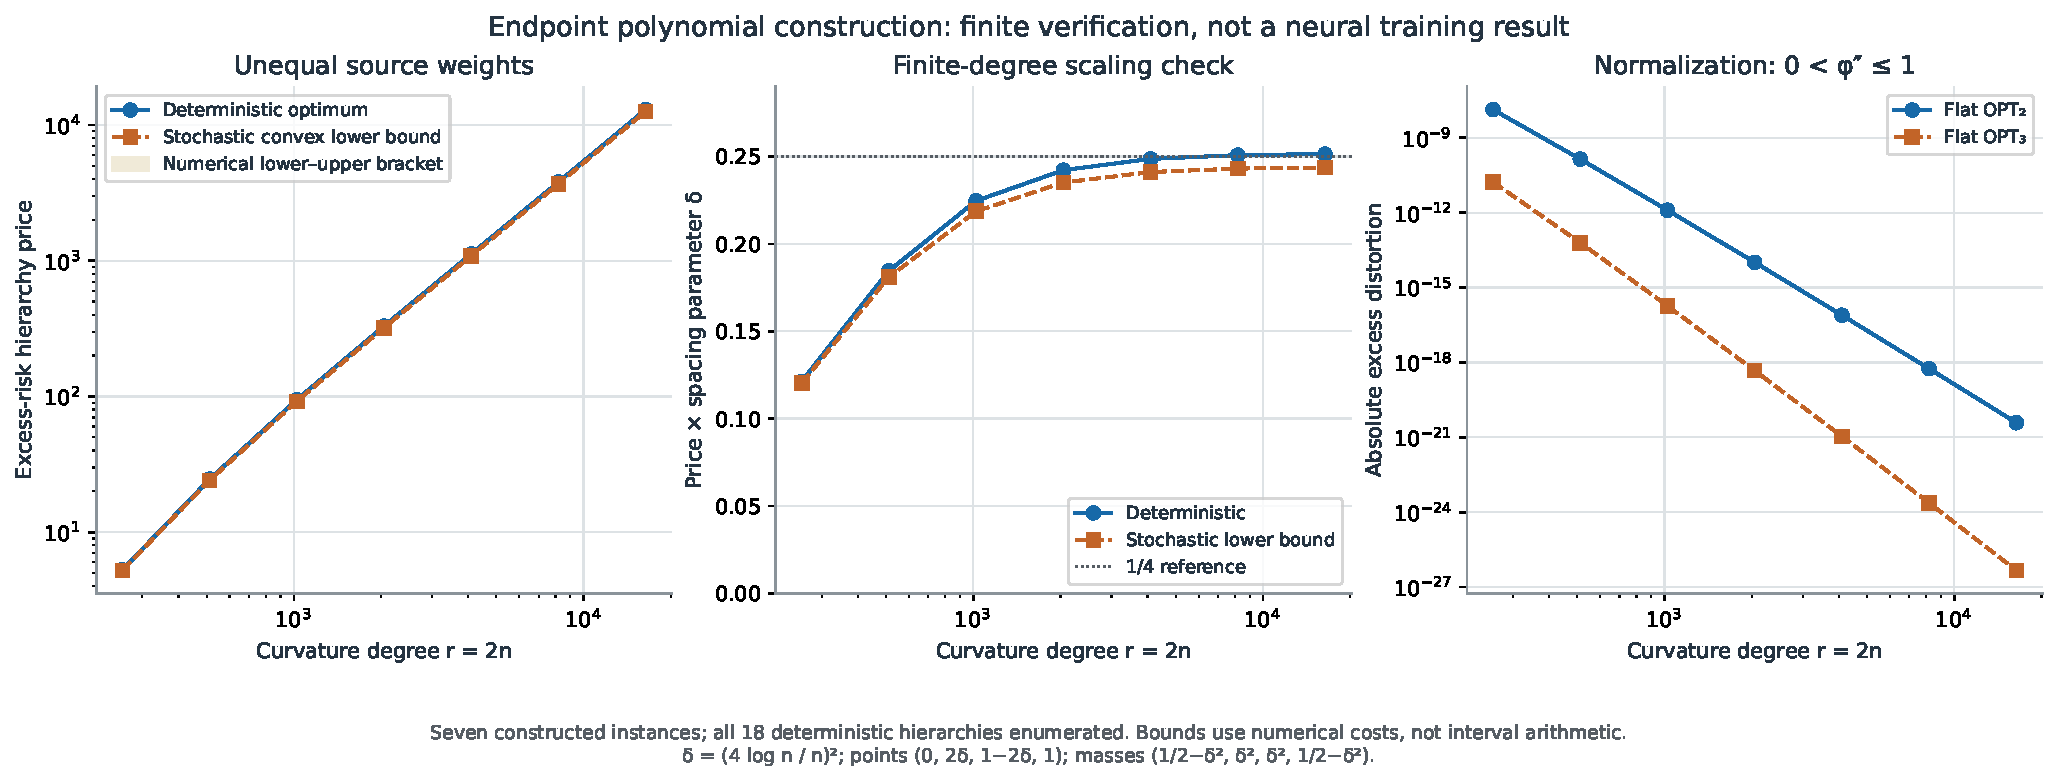
\includegraphics[width=\textwidth]{figures/endpoint_construction.pdf}
\caption{Endpoint family: numerical prices, prices multiplied by
$d_n$ (denoted $\delta$ in the plot), and normalized flat denominators.
The $1/4$ line is a visual reference, not a theorem. All eighteen
deterministic choices are enumerated; floating-point costs are independently
crosschecked as described in the text.}
\label{fig:endpoint}
\end{figure}

\subsection{Equal-mass controls and failed over-localization}
The original interior sequence uses $\varepsilon_n=16\log n/n$ and requires
$\varepsilon_n\le1/16$. The first integer $n\ge2$ meeting that condition is
$1938$, corresponding to curvature degree $7752$. Table~\ref{tab:equalnumerics}
reports the three sampled admissible members of that sequence.

\begin{table}[ht]
\centering\small
\begin{tabular}{@{}rrrrr@{}}
\toprule
$r=4n$ & $\varepsilon_n$ & Deterministic & Stochastic bracket & $n/(32\log n)$ \\
\midrule
8192 & 0.0595673 & 7.26645 & $[4.58790,5.53026]$ & 8.39386 \\
16384 & 0.0324913 & 14.1023 & $[8.07689,9.02771]$ & 15.3887 \\
32768 & 0.0175994 & 27.0290 & $[14.5837,15.5383]$ & 28.4100 \\
\bottomrule
\end{tabular}
\caption{Original equal-mass interior sequence. The last column is its
proved deterministic leading term, not a finite-degree equality. Stochastic
brackets use the convex lower construction and an explicit feasible channel.}
\label{tab:equalnumerics}
\end{table}

The full twenty-eight-case width scan includes distinct control families.
At fixed $\varepsilon=1/16$, price is $1$ at $r=64$, $1.00544$ at $r=128$,
and approaches $6.88889$ at the larger sampled degrees. Increasing degree
with fixed width therefore does not reproduce the diverging sequence.
At $n=8192$, width $\varepsilon_n/4$ gives price $112.170$, whereas the
narrower width $\varepsilon_n/8$ gives only $2.12227$ despite a hinge-reference
prediction of $225.795$. Finite-degree leakage defeats the excessively
narrow construction. These controls are different generators, not
lower-degree members of the original sequence. A separate twenty-four-case
spacing/weight screen contains many compatible instances of price one;
small inner weights alone need not create a conflict for a fixed curvature.

\begin{figure}[ht]
\centering
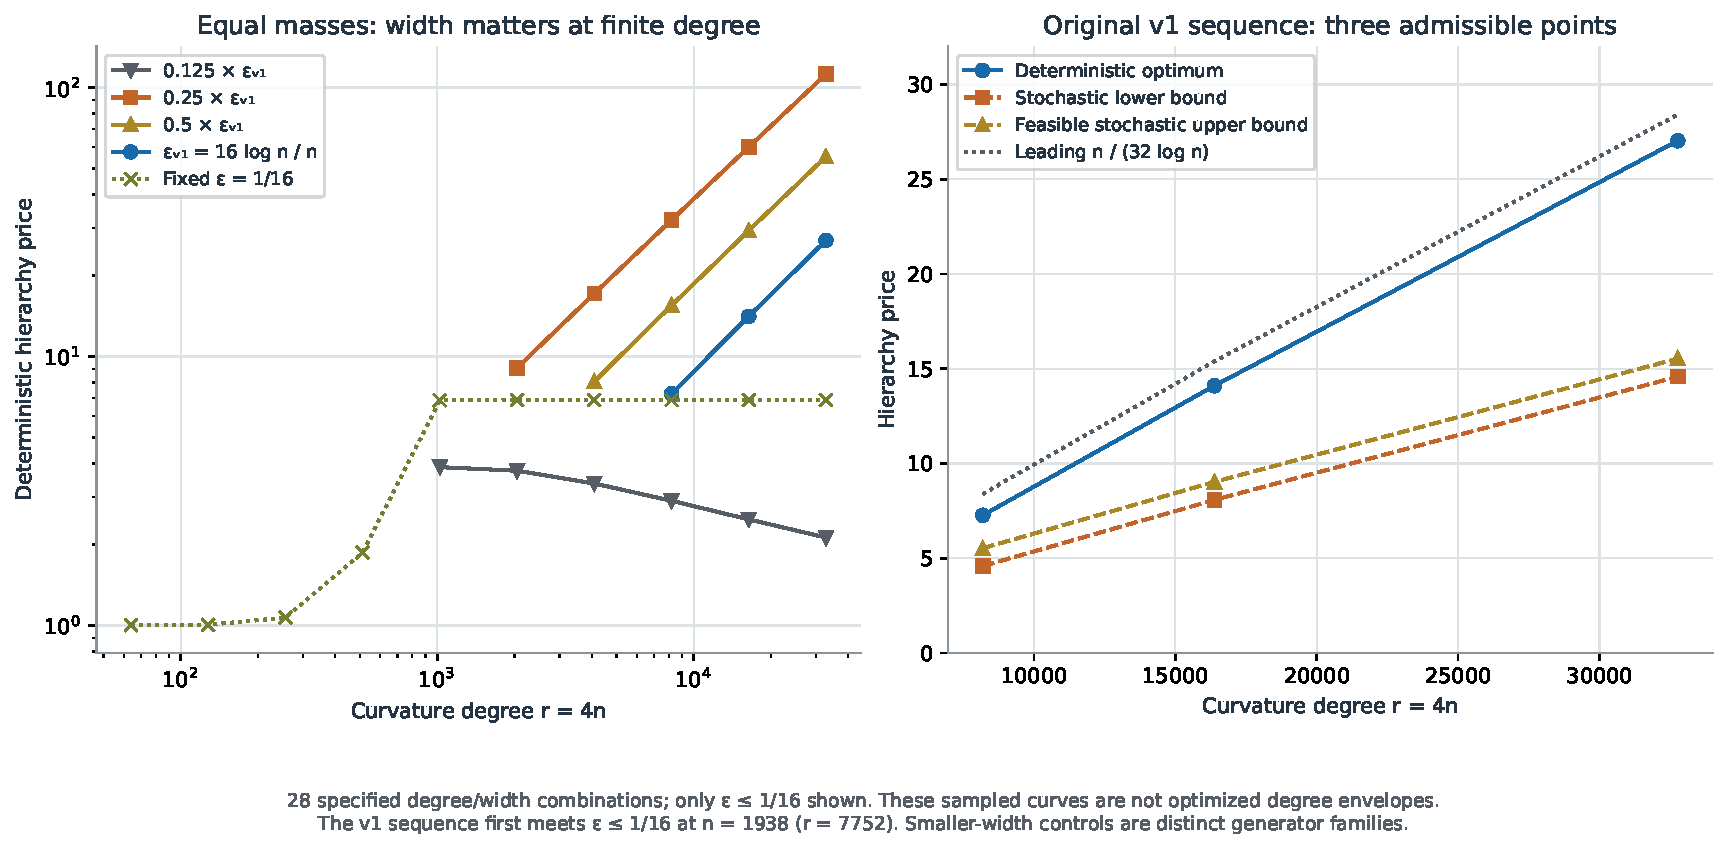
\includegraphics[width=\textwidth]{figures/equal_mass_degree_width.pdf}
\caption{Equal-mass finite-degree controls. The plotted curves are sampled
families, not optimized envelopes. The right panel uses only the three
admissible sampled members of the original interior sequence.}
\label{fig:equalcontrols}
\end{figure}

The uniform upper proof has intentionally loose constants:
$\log K=\log64+100\pi\log512\approx1963.986364$ in
\eqref{eq:logimplicit}. These experiments cannot certify its practical
threshold or either envelope's optimal leading constant. They also do not
numerically test the arbitrary-source all-capacity theorem.

\subsection{Reproduction and the representation-learning interface}
The companion script \path{research/experiments/code/reproduce.sh} reruns
the computations using an already available Python environment; no
installation or training is performed. The actual environment was Python
3.12.14 with NumPy 2.3.5, SciPy 1.18.1, mpmath, and Matplotlib 3.11.2.
Configuration files and logs preserve seeds, commands, environment versions,
and source hashes. Calculations used one main process and one-thread
BLAS/OpenMP caps; the successful recorded numerical phases took about
$31.5$ seconds in total, excluding startup and figure rendering. This is an
execution record rather than a performance benchmark.

The connection to representation learning requires a specified finite
state representation, source masses, Bernoulli posteriors, decoder, and
coarsening relation. If neuron growth is modeled as splitting cells of an
existing partition, the oracle Jensen costs quantify the price of retaining
that partition across capacities. Counting neurons does not itself supply
this finite-output model, and a learned predictor need not achieve the
oracle costs. Neither these calculations nor the hierarchy theorems imply
that a neuron-splitting rule improves training or population risk. A separate
learning experiment would need an explicit optimization and decoder model,
statistical error control, and a data-access and memory budget.


\section{Degree regimes and remaining questions}
\label{sec:conclusion}
The degree-uniform problem separates into the scopes stated in Theorem~\ref{thm:main}. For equal four-state masses,
\begin{equation}
c\frac{r}{\log r}\le C_r^{\stp}\le C_r^{\detp}
\le C\frac{r}{\log r},
\label{eq:mainbounds}
\end{equation}
with absolute constants for sufficiently large $r$. Arbitrarily degenerating posterior gaps are allowed in the upper bound, while the fixed quartet $(1/8,3/8,5/8,7/8)$ attains the lower order. The constructed deterministic and stochastic sequence constants differ by a factor of two; this does not determine the leading constants or their ratio for the separate worst-case envelopes. The explicit Fourier estimates $384r+1728$ and $192r+864$ remain useful finite-degree bounds.

Allowing arbitrary positive weights changes the order that is possible. Writing $\widehat C_r$ for the four-state two-/three-output envelope gives
\[
c\frac{r^2}{(\log r)^2}\le\widehat C_r^{\stp}
\le\widehat C_r^{\detp}\le1+128r^2.
\]
The squared-logarithm gap remains unresolved. Fixed positive weights retain $\Theta_p(r/\log r)$ by comparison, whereas the endpoint witnesses have smallest mass $256(\log n)^4/n^4$ and changing posterior gaps. A sharp joint degree/minimum-mass bound, and a separation of weight degeneration from location degeneration, remain open.

Let $A_r^{\detp}$ and $A_r^{\stp}$ be the corresponding all-capacity envelopes over all finite sources and positive weights. The full four-state witnesses and the uniform curvature-coordinate comparison yield
\[
c\frac{r^2}{(\log r)^2}\le A_r^{\stp}\le A_r^{\detp}
\le256r^2\bigl(2\log(64r^2)+\tfrac14\bigr).
\]
This improves the coarse $O(r^4)$ all-capacity bound to $O(r^2\log r)$. It leaves a logarithmic-cube gap between the displayed lower and upper orders, and does not establish that the upper logarithm is necessary. The coordinate and squared-distance transfer are established tools; the relevant quantitative step is the degree-only comparison for each \emph{oriented} divergence, including curvatures with zeros.

Fixed-generator regularity is a separate issue. Finite-order curvature zeros, including analyticity across the closed interval, give a finite all-capacity bound independent of source size and positive weights. Monotone curvature gives a bound depending on the smallest source mass even with infinite-order endpoint flatness. For smooth curvature positive in the interior, four-equal-mass divergence requires an endpoint that is infinitely flat and persistently nonmonotone. Those conditions are jointly insufficient, so a necessary-and-sufficient characterization remains open.

These are optimal excess-distortion existence statements. They do not guarantee the output of greedy agglomeration or a neural training procedure. Bounded proper-loss normalization preserves price ratios, while absolute distortions can become very small. Connecting the present results to learned representations requires additional statistical and optimization analysis; the experiments supply numerical checks of finite scalar instances only.

\section{Provenance and verification boundaries}
\label{sec:provenance}
\paragraph{Established hierarchy and loss tools.}
The hierarchy-transfer theorem is established work of Lin et al.\ \cite{lin}, checked here through the primary restatement in Gro\ss wendt's thesis \cite[Theorem 2.11]{grosswendt} and the later treatment in Arutyunova and R\"oglin \cite{arutyunova}. The original Lin article's bibliographic record and author-hosted pointer were verified, but its full text could not be obtained; the author-hosted PDF returned an access error. The theorem is therefore invoked through Gro\ss wendt's inspected restatement, without pretending to have checked the original proof. The positive-real-weight Euclidean augmentation calculation is given in Lemma~\ref{lem:hilbert}, rather than inferred by integer replication. Bregman centroids and proper-loss representations have the antecedents cited in Section~\ref{sec:definitions}.

\paragraph{Geometric and polynomial antecedents.}
The coordinate $h=\int\sqrt{\ph''}$ is established in the geometry of separable Bregman divergences \cite{gomes,gzyl}. Original-coordinate similarity \cite{ackermann}, approximate Bregman symmetry for power-type examples \cite{kindermann}, and doubling or engulfing geometry \cite{calogero,maldonado} give related sufficient-condition tools. They do not by themselves supply all the finite-order, endpoint, and hierarchy assertions proved here. Markov's inequality \cite{shadrin}, Chebyshev identities \cite{dlmf}, and positive-polynomial concentration are classical. For example, Levin and Lubinsky \cite[Theorem 1.3]{levin} give interior $L^1$ evaluation estimates through Christoffel functions, while Raikov and Beltukov \cite{raikov} analyze localized positive polynomial kernels. The proof of Theorem~\ref{thm:linearupper} uses an elementary Fourier-coefficient estimate so that the needed concentration bound and its endpoint dependence are explicit. The sharper Theorem~\ref{thm:logupper} uses the classical outer Fej\'er--Riesz factorization as stated by Dritschel and Woerdeman \cite[Introduction]{dritschelwoerdeman}; its radial estimate and Poisson argument, including boundary zeros, are justified in the proof. The squared-Chebyshev kernel in \eqref{eq:chebkernel} has a direct antecedent in Kro\'o and Szabados \cite[Proposition 1]{krooszabados}, who also choose logarithmic-over-degree width. We use this source to credit the needle construction and prove all normalization and tail estimates required here independently.

The endpoint construction in Section~\ref{sec:ext-weights} uses classical external-Chebyshev growth, a different localization scale from the interior squared needle. Endpoint/interior localization distinctions are classical; see Totik \cite[Section 4]{totik} for background. We prove the particular normalization and tail bounds directly, and do not import a stronger endpoint profile from that survey. Section~\ref{sec:poly-allcap-new} uses the established coordinate $h$ but proves a uniform comparison for each oriented divergence. The familiar inequality $|h(v)-h(u)|^2\le (v-u)\int_u^v g$ controls the \emph{symmetrized} divergence and follows by Cauchy--Schwarz; see also \cite[Section 5, Proposition 8]{nielsen}. It does not alone give the oriented logarithmic comparison. Gzyl's comparison theorem requires additional smoothness, nondegeneracy, and sign hypotheses, which are not silently imposed on arbitrary polynomial curvature with zeros.

\paragraph{Prior project construction.}
The fixed smooth obstruction, the hinge reference costs, the deterministic Pareto alternatives, the random-function-table stochastic lower comparison, and the explicit stochastic channel come from the supplied Phase 7 working paper \cite[Section 4]{huang7}. They are reproduced here where needed. Qualitative unboundedness over the union of polynomial degrees already follows from that obstruction and positive polynomial approximation of curvature: for each fixed smooth instance, sufficiently accurate approximation preserves its positive-denominator hierarchy ratios. The present construction supplies a quantitative relation between degree and price, fixed interior posterior locations, and deterministic and stochastic asymptotics. Combined with the uniform upper theorem, it determines the sharp degree order in the four-equal-mass setting; this mathematical statement does not by itself establish historical novelty.

\paragraph{Related clustering and refinement formulations.}
Agglomerative hierarchies for Bregman costs have been studied, including the merge-cost formulation of Telgarsky and Dasgupta \cite{telgarsky}. Their greedy tree construction and the simultaneous-capacity comparison with separately optimal flat solutions studied here are distinct criteria.
Successive refinement of the information bottleneck \cite{charvin} and logarithmic-loss source coding \cite{no} concern related compatibility questions. Their mutual-information or asymptotic rate-distortion constraints differ from the finite output-cardinality and multiplicative excess-risk criterion here. Their results are not used as hierarchy-price bounds in this paper.

\paragraph{Status.}
The mathematical results have undergone internal independent checking, including separate checks of the two extension proofs, together with a bounded primary-literature audit. Neither is external peer review or a certification of novelty. The bounded source review did not identify a theorem with the same quantitative scope as the degree envelopes and oriented polynomial comparison stated here; that observation does not establish priority or an exhaustive literature result. A publication-level novelty assessment would require further citation-chain review, including inspection of the original Lin article. The equal-mass degree order is settled within the stated model. The broader weighted and all-capacity orders, optimal leading constants, and a complete regularity characterization remain unresolved.

\begin{thebibliography}{99}
\small
\bibitem{ackermann}
Marcel R. Ackermann and Johannes Bl\"omer.
\emph{Coresets and Approximate Clustering for Bregman Divergences}.
Revised manuscript, 2009; proceedings version in the Twentieth Annual ACM--SIAM Symposium on Discrete Algorithms.
\url{https://cs.uni-paderborn.de/fileadmin/informatik/fg/cuk/Forschung/Publikationen/CoresetsAndApproximateClusteringForBregmanDivergences.pdf}.

\bibitem{arutyunova}
Anna Arutyunova and Heiko R\"oglin.
The price of hierarchical clustering.
\emph{Algorithmica} 87 (2025), 1420--1452.
\url{https://doi.org/10.1007/s00453-025-01327-7}.

\bibitem{banerjee}
Arindam Banerjee, Srujana Merugu, Inderjit S. Dhillon, and Joydeep Ghosh.
Clustering with Bregman divergences.
\emph{Journal of Machine Learning Research} 6 (2005), 1705--1749.
\url{https://www.jmlr.org/papers/volume6/banerjee05b/banerjee05b.pdf}.

\bibitem{calogero}
A. Calogero and R. Pini.
The engulfing property for sections of convex functions on the Heisenberg group and the associated quasi-distance.
\emph{Journal of Geometric Analysis}, online publication, 2021.
\url{https://doi.org/10.1007/s12220-021-00648-7}.

\bibitem{charvin}
Hippolyte Charvin, Nicola Catenacci Volpi, and Daniel Polani.
Exact and soft successive refinement of the information bottleneck.
\emph{Entropy} 25 (2023), 1355.
\url{https://doi.org/10.3390/e25091355}.

\bibitem{dritschelwoerdeman}
Michael A. Dritschel and Hugo J. Woerdeman.
\emph{Outer Factorizations in One and Several Variables}.
Preprint, 2004, arXiv:math/0403099; Introduction for the classical scalar theorem.
\url{https://arxiv.org/abs/math/0403099}.

\bibitem{gneiting}
Tilmann Gneiting and Adrian E. Raftery.
Strictly proper scoring rules, prediction, and estimation.
\emph{Journal of the American Statistical Association} 102(477) (2007), 359--378.
\url{https://doi.org/10.1198/016214506000001437}.

\bibitem{gomes}
Erika Gomes-Gon\c calves, Henryk Gzyl, and Frank Nielsen.
\emph{Geometry and Clustering with Metrics Derived from Separable Bregman Divergences}.
Preprint, 2018, arXiv:1810.10770.
\url{https://arxiv.org/abs/1810.10770}.

\bibitem{grosswendt}
Anna-Klara Gro\ss wendt.
\emph{Theoretical Analysis of Hierarchical Clustering and the Shadow Vertex Algorithm}.
Doctoral thesis, University of Bonn, 2020.
\url{https://d-nb.info/121830152X/34}.

\bibitem{gzyl}
Henryk Gzyl.
\emph{From Generalized Arithmetic Means to Geodesics to Hamilton Dynamics to Bregman Divergences}.
Preprint, 2020, arXiv:2007.15473.
\url{https://arxiv.org/abs/2007.15473}.

\bibitem{huang7}
Wenyu Huang.
\emph{Exact Residual-Query Memory and Smooth-Loss Hierarchy Limits}.
Unpublished Phase 7 working paper, University of California San Diego, 2026.
Supplied project manuscript; Section 4.

\bibitem{kindermann}
Stefan Kindermann.
A note on the approximate symmetry of Bregman distances.
\emph{Journal of Convex Analysis} 26(3) (2019), 991--999.
\url{https://arxiv.org/abs/1808.06790}.

\bibitem{krooszabados}
Andr\'as Kro\'o and J\'ozsef Szabados.
Polynomial inequalities with asymmetric weights.
\emph{Ja\'en Journal on Approximation} 10 (2018), 81--100.
Repository manuscript, Proposition 1 and its proof; construction attribution only, with the estimates needed here proved independently.
\url{https://real.mtak.hu/102404/1/asym.new.pdf}.

\bibitem{levin}
Eli Levin and Doron S. Lubinsky.
$L^p$ Christoffel functions, $L^p$ universality, and Paley--Wiener spaces.
\emph{Journal d'Analyse Math\'ematique} 125 (2015), 243--283.
\url{https://doi.org/10.1007/s11854-015-0008-2}.

\bibitem{lin}
Guolong Lin, Chandrashekhar Nagarajan, Rajmohan Rajaraman, and David P. Williamson.
A general approach for incremental approximation and hierarchical clustering.
\emph{SIAM Journal on Computing} 39(8) (2010), 3633--3669.
\url{https://doi.org/10.1137/070698257}.

\bibitem{maldonado}
Diego Maldonado and Colin Williams.
\emph{Geometric Characterizations of H\"older-continuous Quasi-distances and Applications}.
Author-hosted revised manuscript.
\url{https://www.math.ksu.edu/~dmaldona/papers/Holder_quasi_distances_revised.pdf}.

\bibitem{no}
Albert No.
Universality of logarithmic loss in successive refinement.
\emph{Entropy} 21(2) (2019), 158.
\url{https://doi.org/10.3390/e21020158}.

\bibitem{dlmf}
National Institute of Standards and Technology.
\emph{Digital Library of Mathematical Functions}.
Section 18.5, explicit representations of classical orthogonal polynomials, especially Eq.~18.5.1.
\url{https://dlmf.nist.gov/18.5}.

\bibitem{plaxton}
C. Greg Plaxton.
Approximation algorithms for hierarchical location problems.
\emph{Journal of Computer and System Sciences} 72(3) (2006), 425--443.
\url{https://www.cs.utexas.edu/~plaxton/pubs/2006/jcss.pdf}.

\bibitem{raikov}
I. O. Raikov and Y. M. Beltukov.
The kernel polynomial method based on Jacobi polynomials.
\emph{Applied Mathematics and Computation} 490 (2025), 129207.
\url{https://arxiv.org/abs/2407.03328}.

\bibitem{reid}
Mark D. Reid and Robert C. Williamson.
Information, divergence and risk for binary experiments.
\emph{Journal of Machine Learning Research} 12 (2011), 731--817.
\url{https://www.jmlr.org/papers/volume12/reid11a/reid11a.pdf}.

\bibitem{shadrin}
A. Shadrin.
\emph{Twelve Proofs of the Markov Inequality}.
Author-hosted exposition.
\url{https://www.damtp.cam.ac.uk/user/na/people/Alexei/papers/markov.pdf}.
\bibitem{telgarsky}
Matus Telgarsky and Sanjoy Dasgupta.
Agglomerative Bregman clustering.
In \emph{Proceedings of the 29th International Conference on Machine Learning}, 2012.
Proposition 3.8 and Section 6 of the author manuscript.
\url{https://cseweb.ucsd.edu/~dasgupta/papers/relabreg.pdf}.

\bibitem{totik}
Vilmos Totik.
Fast decreasing and orthogonal polynomials.
\emph{Contemporary Mathematics} 578 (2012), 241--254.
Author survey, Section 4, Theorem 4.1; the underlying Totik--Varga original was not separately inspected.
\url{https://www.math.u-szeged.hu/pot/4madridpaper.pdf}.

\bibitem{nielsen}
Frank Nielsen.
Approximation and bounding techniques for the Fisher--Rao distances between parametric statistical models.
\emph{Handbook of Statistics} 51 (2024), 67--116.
Inspected arXiv version 4, 7 January 2025, Section 5, Proposition 8.
\url{https://arxiv.org/pdf/2403.10089v4}.
\end{thebibliography}
\end{document}
